% mnras_template.tex
%
% LaTeX template for creating an MNRAS paper
%
% v3.0 released 14 May 2015
% (version numbers match those of mnras.cls)
%
% Copyright (C) Royal Astronomical Society 2015
% Authors:
% Keith T. Smith (Royal Astronomical Society)

% Change log
%
% v3.0 May 2015
%    Renamed to match the new package name
%    Version number matches mnras.cls
%    A few minor tweaks to wording
% v1.0 September 2013
%    Beta testing only - never publicly released
%    First version: a simple (ish) template for creating an MNRAS paper

%%%%%%%%%%%%%%%%%%%%%%%%%%%%%%%%%%%%%%%%%%%%%%%%%%
% Basic setup. Most papers should leave these options alone.
\documentclass[a4paper,fleqn,usenatbib]{mnras}

% MNRAS is set in Times font. If you don't have this installed (most LaTeX
% installations will be fine) or prefer the old Computer Modern fonts, comment
% out the following line
\usepackage{newtxtext,newtxmath}
% Depending on your LaTeX fonts installation, you might get better results with one of these:
%\usepackage{mathptmx}
%\usepackage{txfonts}

% Use vector fonts, so it zooms properly in on-screen viewing software
% Don't change these lines unless you know what you are doing
\usepackage[T1]{fontenc}
\usepackage{ae,aecompl}


%%%%% AUTHORS - PLACE YOUR OWN PACKAGES HERE %%%%%

% Only include extra packages if you really need them. Common packages are:
\usepackage{graphicx}	% Including figure files
\usepackage{amsmath}	% Advanced maths commands
\usepackage{amssymb}	% Extra maths symbols
\usepackage{subfig}
%%%%%%%%%%%%%%%%%%%%%%%%%%%%%%%%%%%%%%%%%%%%%%%%%%

%%%%% AUTHORS - PLACE YOUR OWN COMMANDS HERE %%%%%

% Please keep new commands to a minimum, and use \newcommand not \def to avoid
% overwriting existing commands. Example:
%\newcommand{\pcm}{\,cm$^{-2}$}	% per cm-squared

%%%%%%%%%%%%%%%%%%%%%%%%%%%%%%%%%%%%%%%%%%%%%%%%%%

%%%%%%%%%%%%%%%%%%% TITLE PAGE %%%%%%%%%%%%%%%%%%%

% Title of the paper, and the short title which is used in the headers.
% Keep the title short and informative.
\title[Title]{The expected shape of the Milky Way's Dark Matter halo}

% The list of authors, and the short list which is used in the headers.
% If you need two or more lines of authors, add an extra line using \newauthor
\author[Jesus Prada,  Jaime E. Forero-Romero, Volker Springel ]{
Jesus Prada,$^{1}$\thanks{E-mail: jd.prada1760@uniandes.edu.co}
Jaime E. Forero-Romero,$^{1}$
Volker Springel$^{2}$
\\
% List of institutions
$^{1}$Departamento de Física, Universidad de los Andes, Cra. 1 No.
18A-10, Edificio Ip, Bogotá, Colombia.\\
$^{2}$Heidelberg Institute for Theoretical Studies, Schloss-Wolfsbrunnenweg 35, D-69118 Heidelberg
Germany.\\
}

% These dates will be filled out by the publisher
\date{Accepted XXX. Received YYY; in original form ZZZ}

% Enter the current year, for the copyright statements etc.
\pubyear{2018}

% Don't change these lines
\begin{document}
\label{firstpage}
\pagerange{\pageref{firstpage}--\pageref{lastpage}}
\maketitle

% Abstract of the paper
\begin{abstract}
This is a simple template for authors to write new MNRAS papers.
The abstract should briefly describe the aims, methods, and main results of the paper.
It should be a single paragraph not more than 250 words (200 words for Letters).
No references should appear in the abstract.
\end{abstract}

% Select between one and six entries from the list of approved keywords.
% Don't make up new ones.
\begin{keywords}
keyword1 -- keyword2 -- keyword3
\end{keywords}

%%%%%%%%%%%%%%%%%%%%%%%%%%%%%%%%%%%%%%%%%%%%%%%%%%

%%%%%%%%%%%%%%%%% BODY OF PAPER %%%%%%%%%%%%%%%%%%

\section{Introduction}

This is a simple template for authors to write new MNRAS papers.
See \texttt{mnras\_sample.tex} for a more complex example, and \texttt{mnras\_guide.tex}
for a full user guide.

All papers should start with an Introduction section, which sets the work
in context, cites relevant earlier studies in the field by \citet{Others2013},
and describes the problem the authors aim to solve \citep[e.g.][]{Author2012}.

\section{Numerical Simulations}
In this work we use the results of the state-of-the art Auriga simulations \cite{auriga}. It selected a set of 30 isolated halos from the Evolution and Assembly of GaLaxies and their Environments (EAGLE) project \cite{Eagle}. Each halo was identified with the algorithm "Friend of Friends" (FOF) \cite{Davis_et_al._1985}, that recursively links particles if they are closer than some distance threshold referred as linking length. EAGLE follows the evolution of fixed-mass particles of $m_{\text{DM}} = 1.15\cdot 10^7\text{M}_{\odot}$ from $z=127$ to $z=0$, adopting the $\Lambda$CDM model from the \cite[Planck Collaboration et al. (2014)]{Planck_Collaboration_2014}, which is characterized by the parameters: $\Omega_\Lambda=0.693$, $\Omega_\text{m}=0.307$, $\Omega_\text{b}=0.048$ \& $\text{H}_0=67.77\text{kms} ^{-1}\text{Mpc}^{-1}$. 

These halos were randomly selected from a sample of the most isolated quartile of halos whose virial mass $M_{200}$ varied between $10^{12}M_\odot$ and $2\cdot 10^{12}M_\odot$. \textbf{This mass is defined as the mass enclosed within the virial radius $R_{200}$ at which the density becomes 200 times the critical density of the universe. \huge FOOTNOTE \normalsize}. These halos were re-simulated with the (AREPOOO HERE) by increasing the mass resolution of the particles belonging to them and diminishing the resolution of the rest of the particles. This would efficiently simulate external gravitational effects over the studied structure while focusing on a high-resolution version of it.\\

Various versions of the same halo were simulated for different degrees of realism. All 30 halos were simulated within a level-4-degree of resolution defined for Aquarius simulations corresponding to $\tilde 3\cdot 10^6$ high resolution particles of $\tilde 2.5 \cdot 10^5 M_\odot$. The principal details of each of these halos are consigned on the table \ref{tab:level4}. From these halos, 6 of them where re-simulated at level 3 (higher) resolution taking into account a spatial factor of 2 in each dimension. For more information about level 3 halos, their details are printed on table \ref{tab:level3}. Furthermore, fore each halo in each level of resolution there are two versions of the simulation. One of tracks the evolution of DM-only particles while the remaining one evolves DM and baryions with magneto-hydrodynamical (MHD) physics, including DM.\\


\section{Determining the halo shape}

%\subsection{The solid ellipsoid method}

The discretization of the DM density field into particles makes it difficult  to perform some calculations that would require a more continuous distribution. Therefore, there is no trivial way to calculate the DM halo shape at a determined radius. There are different approaches \textbf{ \large ISODENSITY, ISOPOTENTIAL, potential gets rounder, cite binney \normalsize }
\textbf{\large Talk about difference between volume method and isodensity contour at least for DM halos \normalsize} \cite{Vera-Ciro_et_al._2011}. In this work we follow the guidelines by \cite[Vera-Ciro et al. 2011]{Vera-Ciro_et_al._2011} which includes the use of the shape method proposed by \cite[Allgood et al. 2006]{Allgood_et_al._2006}.\\

To calculate the DM halo shape, we initially consider particles enclosed within a sphere of radius $r$. We calculate the reduced inertia tensor:

\begin{equation}
I_{ij} = \sum_k \frac{x_k^{(i)}x_k^{(j)}}{d^2_k},
\label{eq:inertia}
\end{equation}

whose components are weighted by the distance $d^2=x^2+y^2+z^2$, so that each particle contribute with same importance to the sum regardless of their radius from the center.\\

The diagonalization of this tensor yields the principal axes of the structure, as well as the eigen-quantities which are proportional to the squared principal axes $a>b>c$. \textbf{\large SUMARIZE \normalsize} However, if we characterize an ellipsoid taking into account only particles enclosed within a sphere, we are effectively miscalculating its triaxiality \cite{Allgood_et_al._2006}. For this reason, we iteratively recalculate the inertia tensor taking into account the previously characterized ellipsoid.\\

AllGood et al. propose to use the eigenvalues $a>b>c$ and their respective eigen-axes $v_a,v_b,v_c$ to recalculate the inertia tensor over the particles enclosed by the ellipsoid with principal axes (along the respective eigenvectors) equal to $r,r/q,r/s$, where ere $q = b/a$ and $s=c/a$ are the axial ratios. In other words, we repeat the process of calculating the inertia matrix by taking into account particles within an ellipsoid with axial ratios given by the previous diagonalization. In this case, as the constant of proportionality is a free parameter, we choose to hold the size (not the direction) of the principal axis constant.\\

This method looks reliable and it would eventually converge to a more accurate characterization of the halo ellipsoid. However, we are computing the reduced inertia tensor by weighting the contributions with the spherical-metric distance $d^2=x^2+y^2+z^2$, where particles within the same spherical surface are given the same importance. This means we are again introducing some error in the triaxiality of the structure. For this reason, on each iteration we must calculate the inertia tensor taking into account an elliptic metric: $\bar{d}^2 = x^2+y^2/q^2+z^2/s^2$, assuming $x,y,z$ are the corresponding principal axes.\\

In case this concept of an elliptic metric is difficult to grasp, let us consider that, instead of converting the initial enclosing sphere to the halo ellipse, we are converting the halo ellipsoid into a sphere by performing scale transforms along the respective eigen-axes. From this point of view, we start our first-guess calculation of the ellipsoid by computing the reduced inertia tensor \eqref{eq:inertia} for particles enclosed within a sphere of radius $r$. Then with the results of this first guess, we perform the following scale transform:
  
\begin{align}
(x,y,z) &\rightarrow (x',y',z')=(x,y/q,z/s) \label{eq:scale}\\
q &=  b/a \nonumber \\
s &= c/a \nonumber ,
\end{align}

where we assumed the unit vectors $\hat{x},\hat{y},\hat{z}$ are oriented at the principal elliptic axes. We then repeat the process of calculating the reduced inertia tensor and performing the scale transformation until we achieve a certain convergence criterion. We stop this iterative process when the sum of the fractional change in axes is less than $10^{-6}$. Finally, we obtain the shape of the halo at the geometric mean radius $(abc)^{1/3}$, which is not much different from the initial radius.\\

Notice that, for diagonalization purposes, calculating the inertia tensor with the scaled coordinates $x',y',z'$ is equivalent to calculating it with the un-scaled coordinates $x,y,z$, using the elliptic-metric distance $\bar{d}^2 = x^2+y^2/q^2+z^2/s^2$.\\



\section{Results}
Here we present our principal results blah blah blah.

\subsection{The radial tendency of axial ratios}
First, it is important to verify that halos are rounder at larger radii, for both MHD and DM simulations.

\begin{figure}
  \centering
  \subfloat[halo 27 DM shape at small radius]{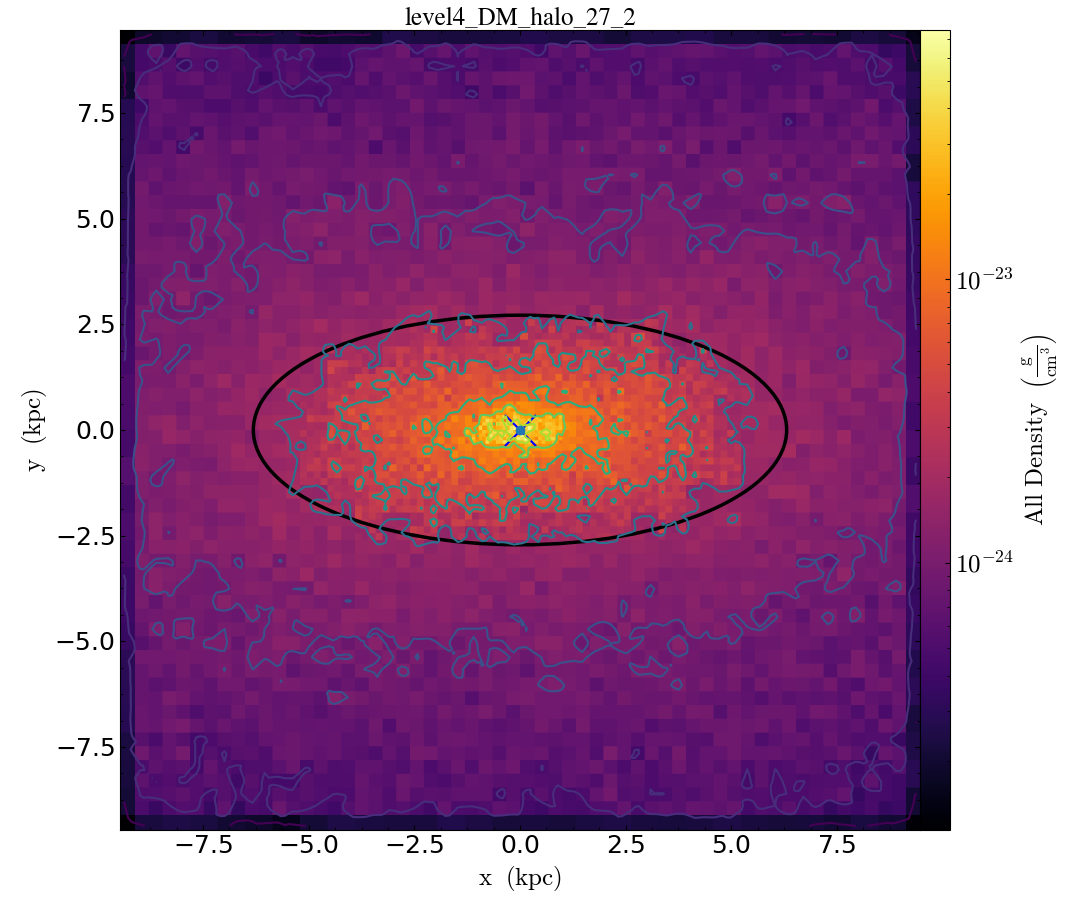
\includegraphics[width=0.5\columnwidth]{./pics/MHD_Vs_DM/level4_DM_halo_27_inner.png}}
  \hfill
  \subfloat[halo 27 DM shape at big radius]{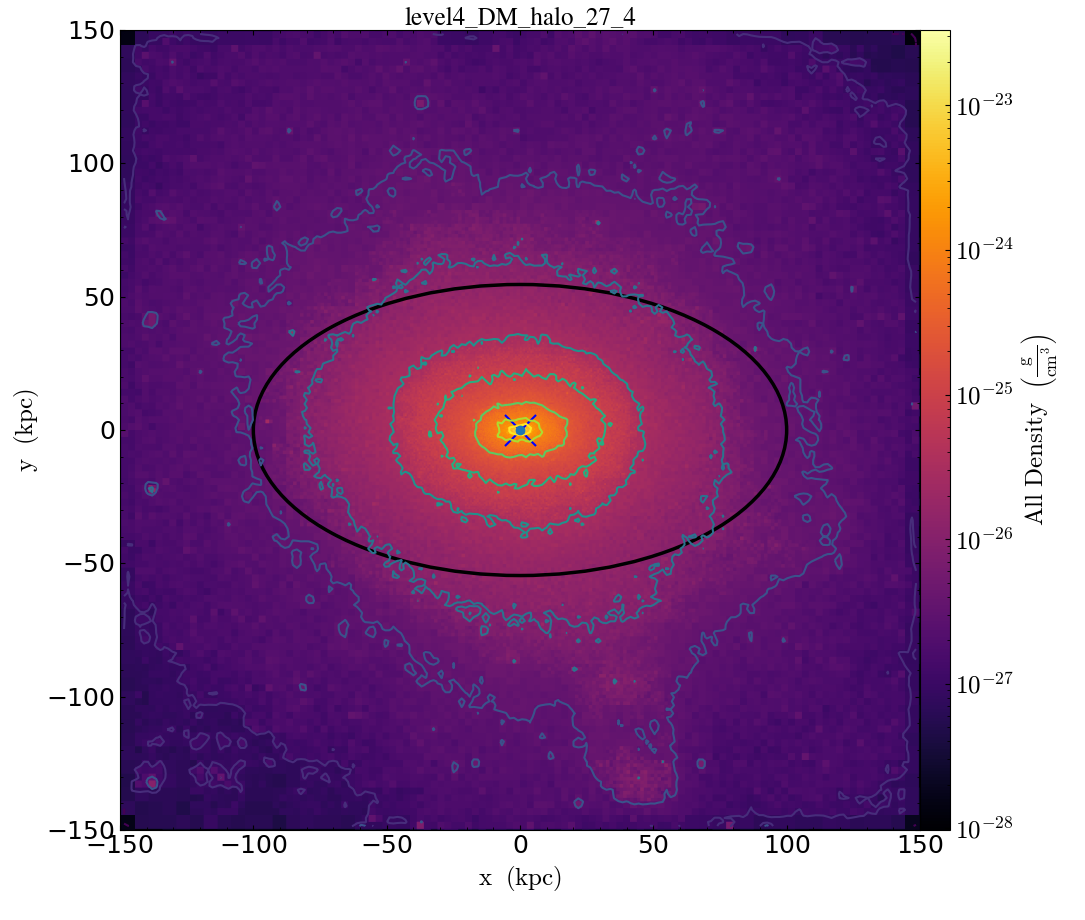
\includegraphics[width=0.5\columnwidth]{./pics/MHD_Vs_DM/level4_DM_halo_27_outter.png}}
  \hfill
  \subfloat[halo 27 MHD shape at small radius]{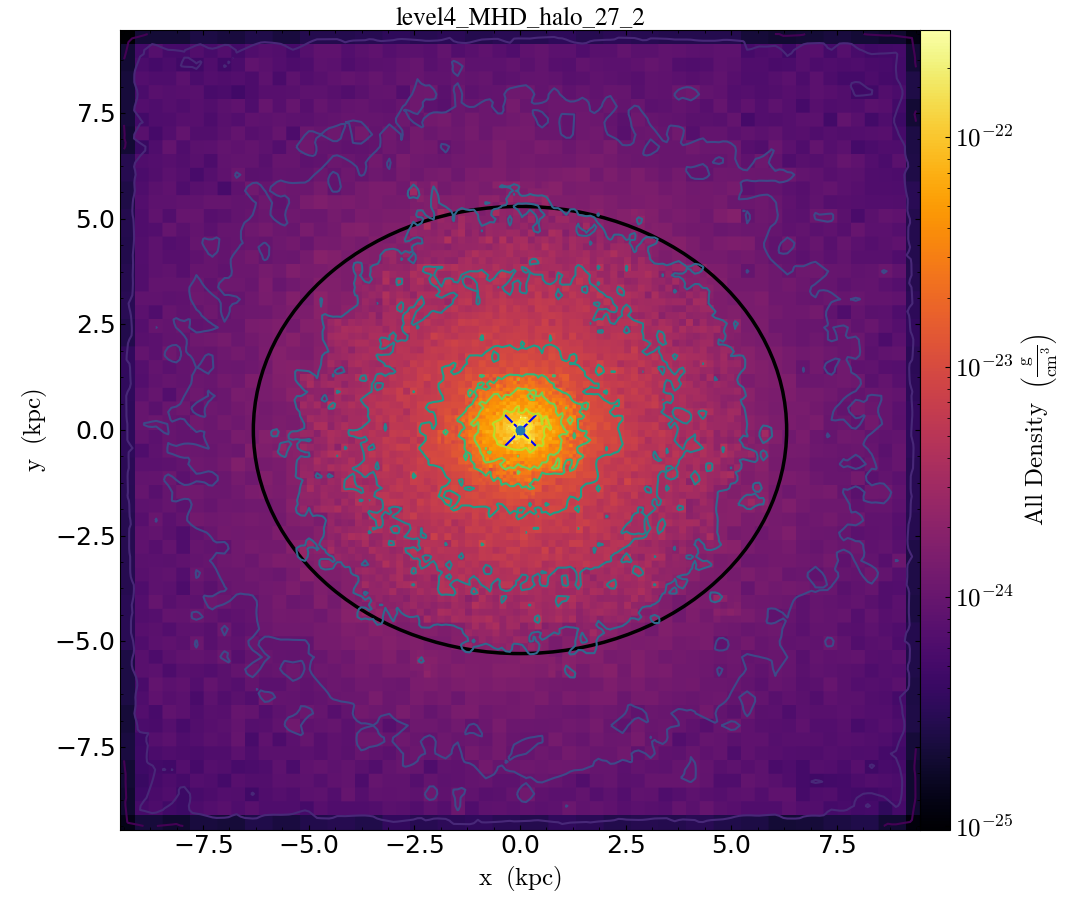
\includegraphics[width=0.5\columnwidth]{./pics/MHD_Vs_DM/level4_MHD_halo_27_inner.png}}
  \hfill
  \subfloat[halo 27 MHD shape at big radius]{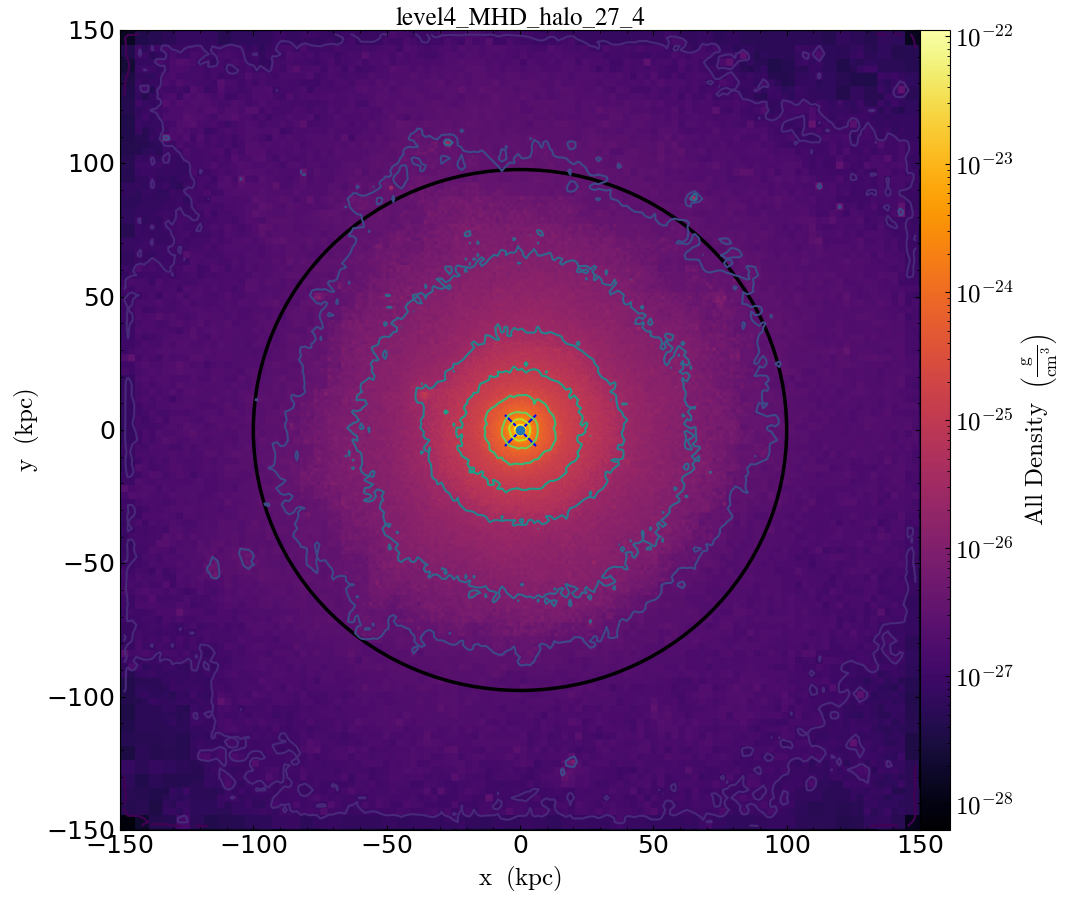
\includegraphics[width=0.5\columnwidth]{./pics/MHD_Vs_DM/level4_MHD_halo_27_outter.png}}
  \caption{DM density for inner (left) and outer (right) parts of the halo 27. We present both versions of the halo: DM (up) \& MHD (down). The horizontal (vertical) axes are aligned to the major (medium) axes. (optimaze space and description) }
  \label{fig:slices}
\end{figure}

\begin{figure}
\centering
\subfloat[halo 16]{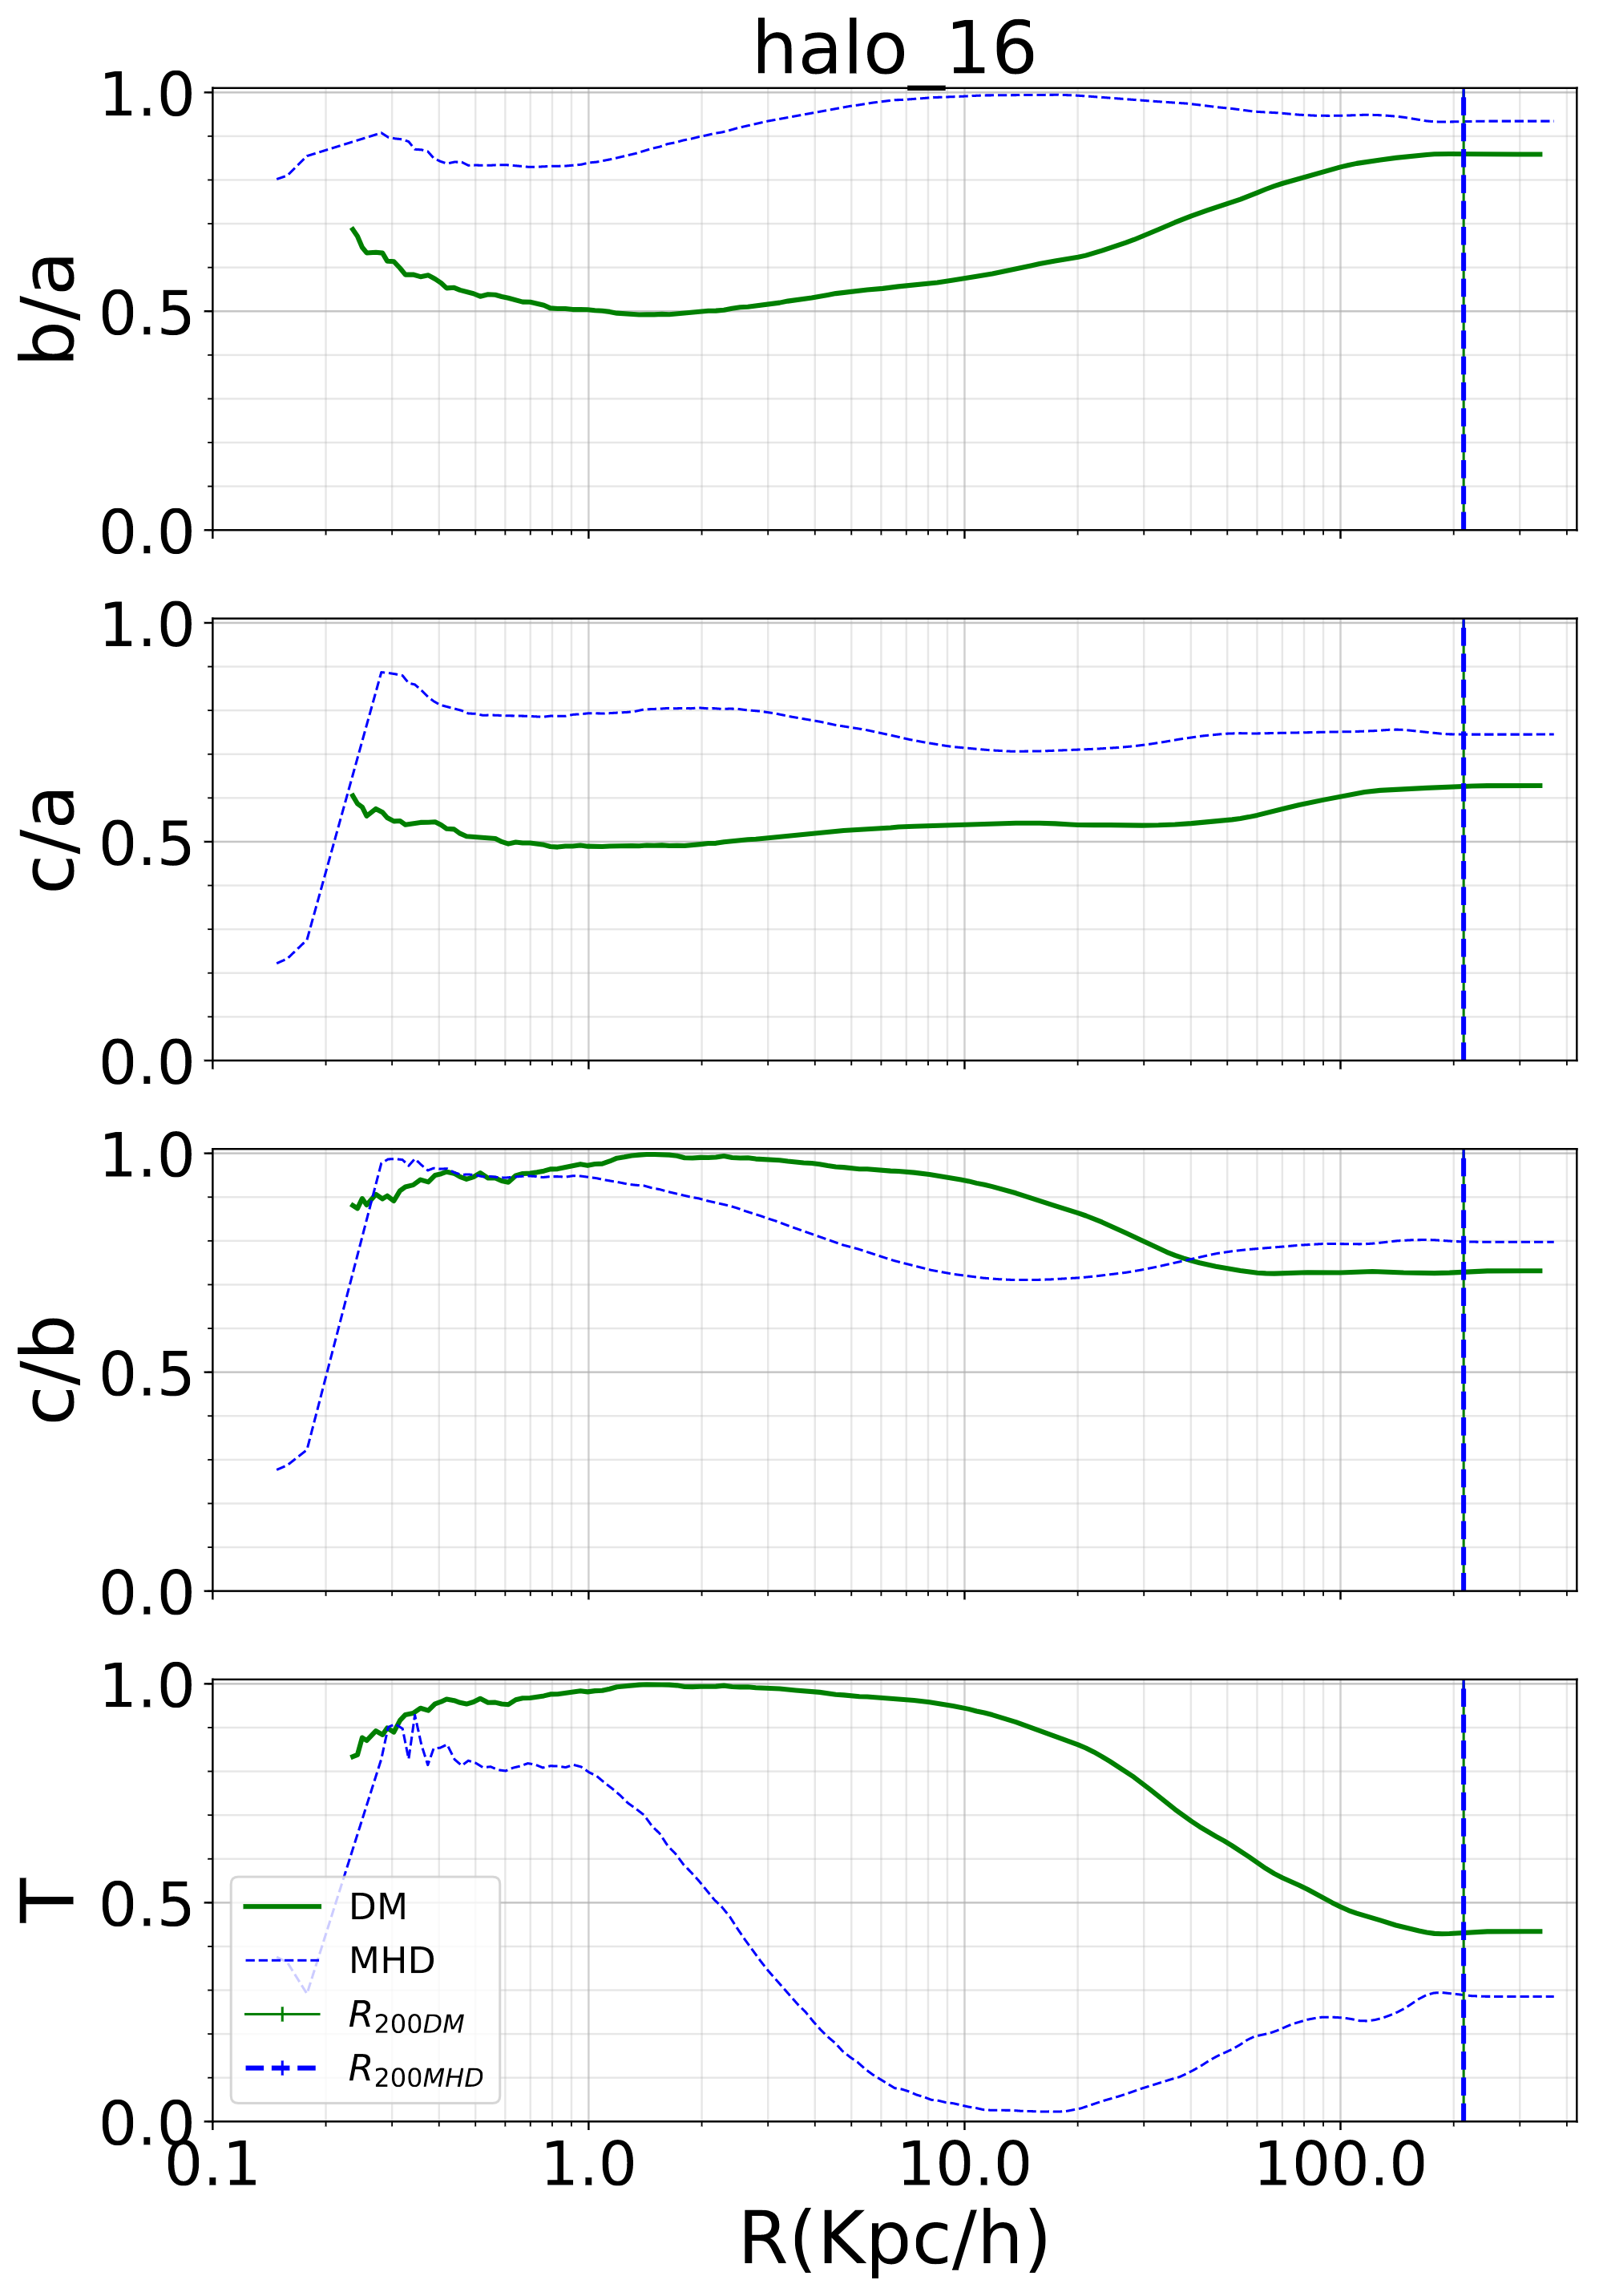
\includegraphics[width=0.5\columnwidth]{./pics/halo16.png}}
  \hfill
  \subfloat[halo 27]{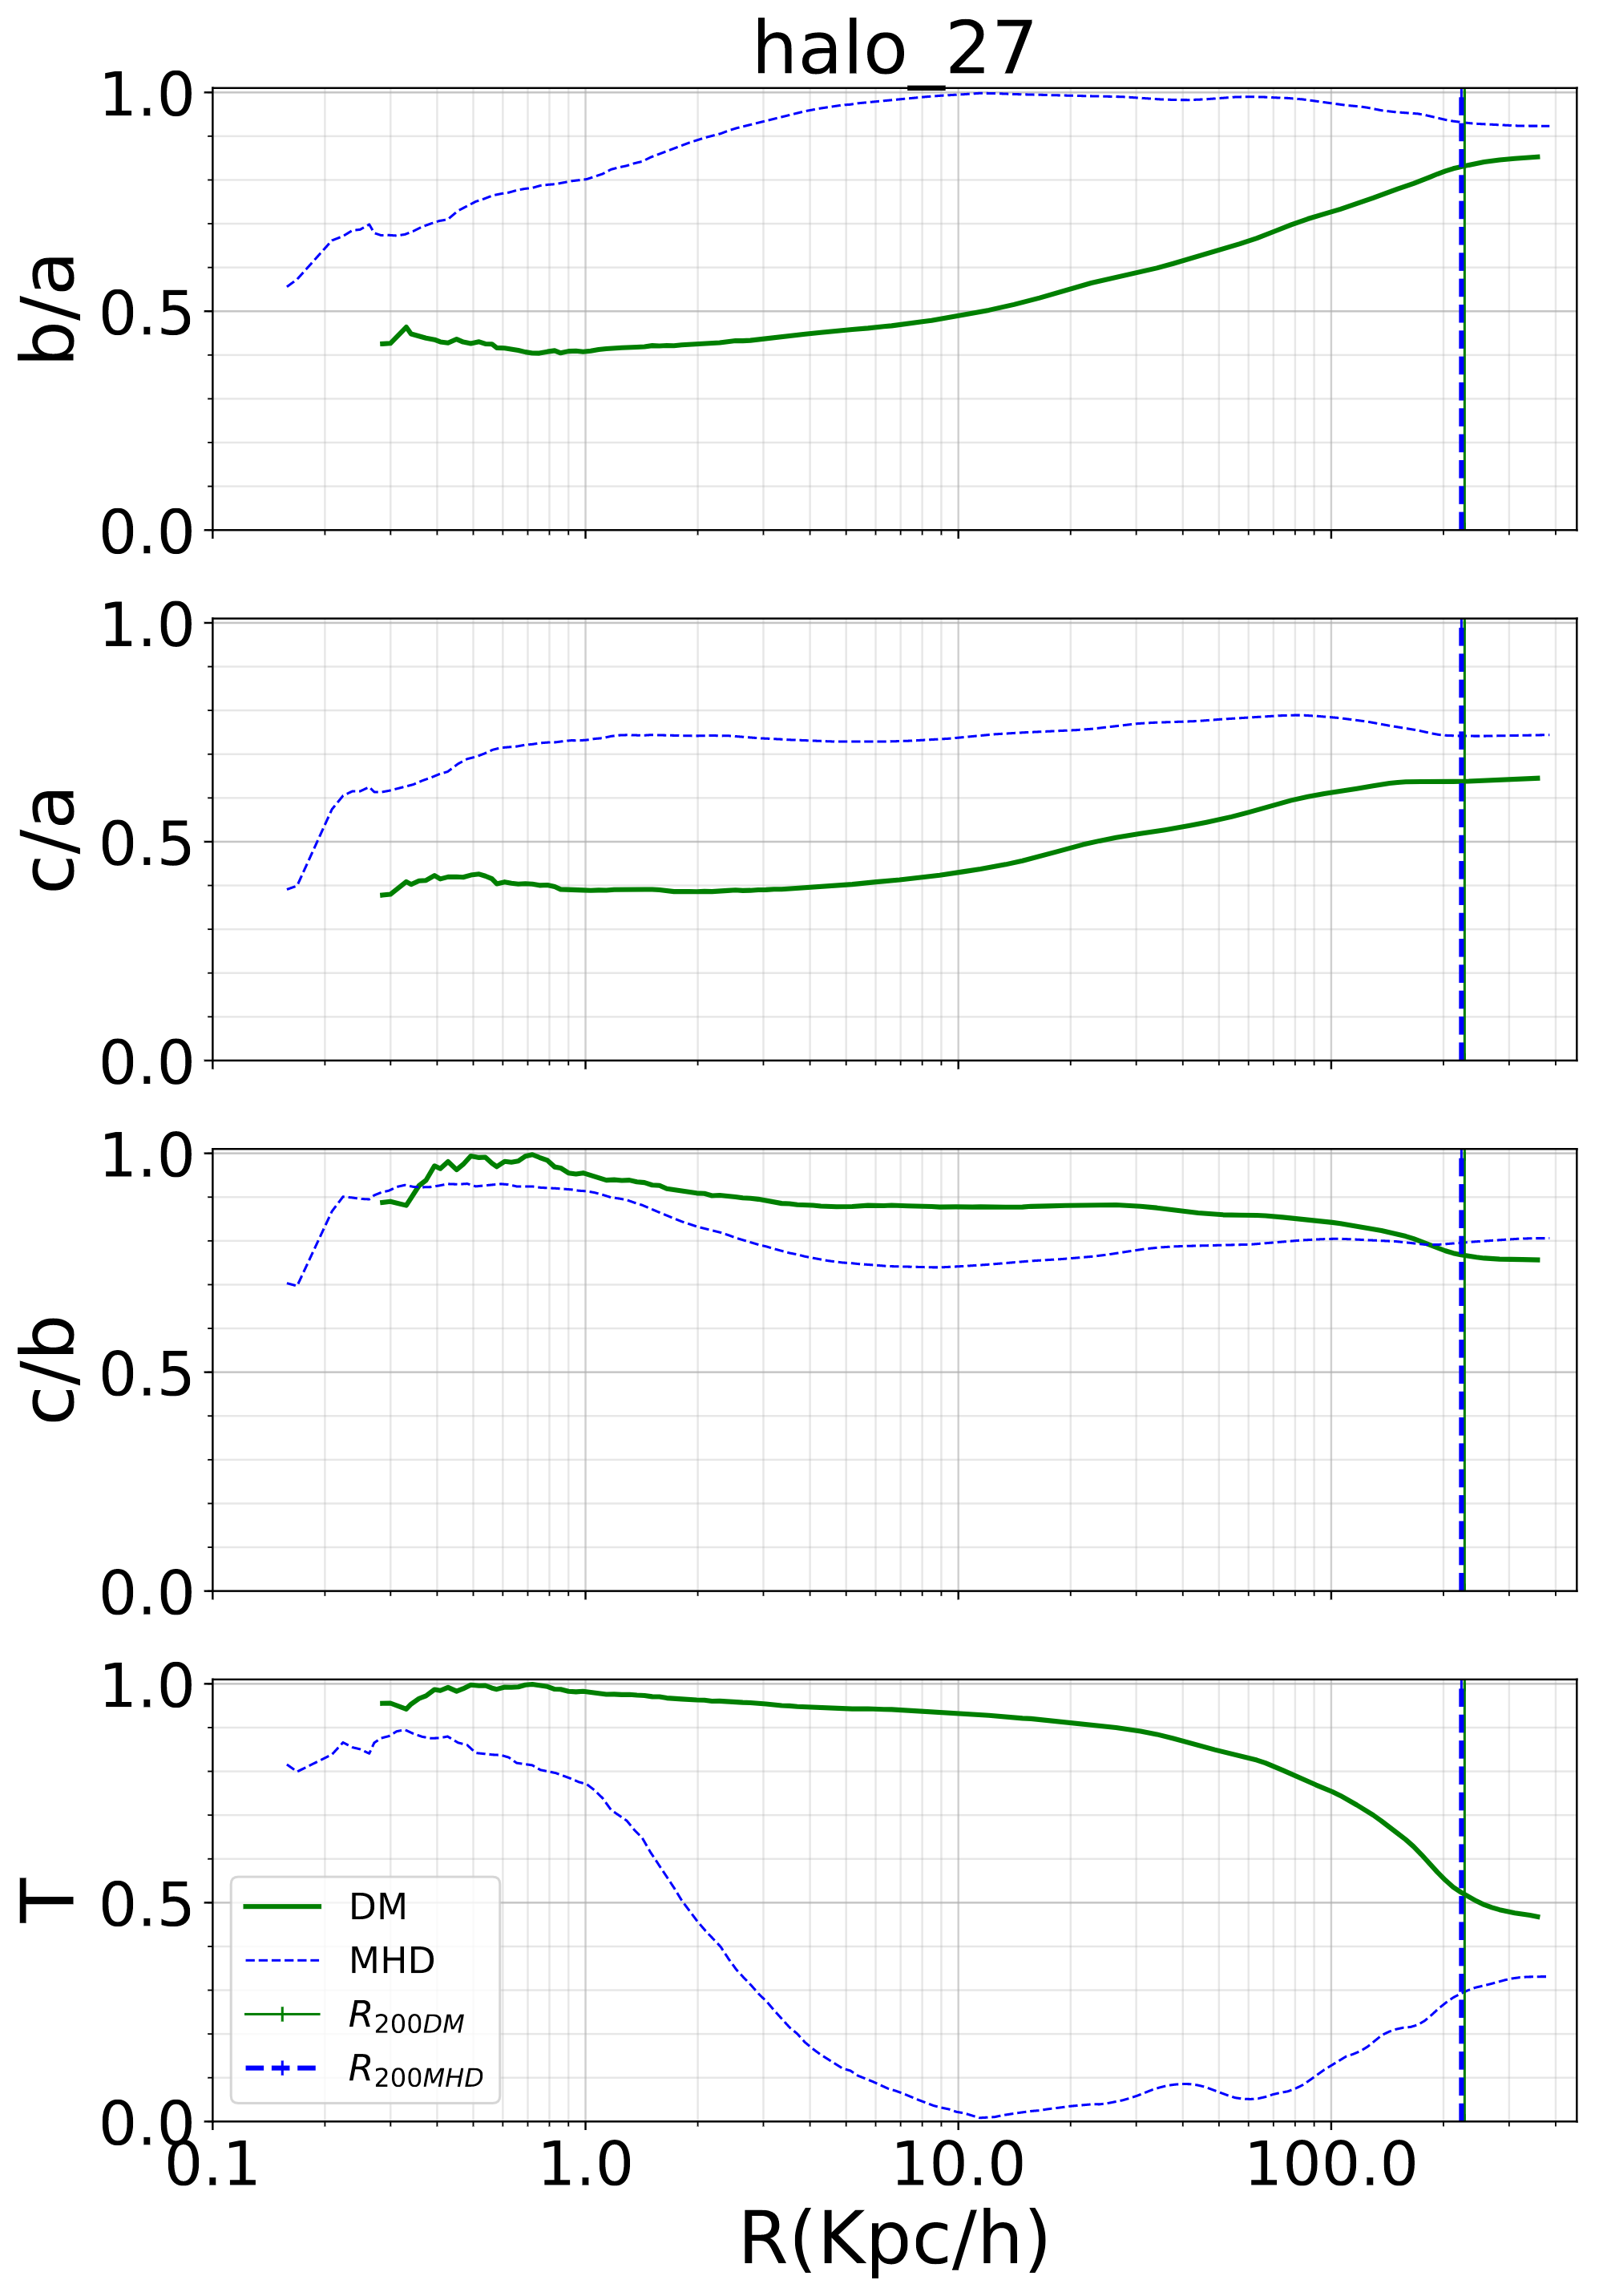
\includegraphics[width=0.5\columnwidth]{./pics/halo27.png}}
\caption{Radial profile for axial ratios and the triaxiality parameter $T=\frac{1-b/a}{1-c/a}$ from halo 27 and halo 16. These halos have a clear radial tendence towards sphericity (for smaller radii until $\approx 3$Kpc), which can be confirmed with the triaxiality parameter. (Merged Column)}
\label{fig:DM_MHD}
\end{figure} 

\begin{figure}
  \centering
  \subfloat[Level4 DM inner Vs outer regions]{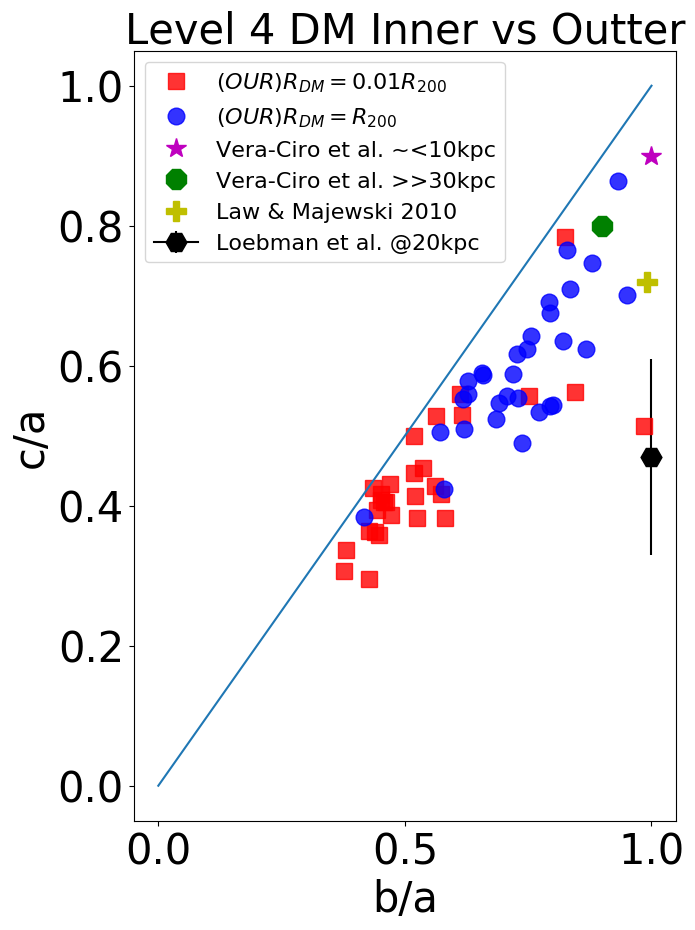
\includegraphics[width=0.5\columnwidth]{./pics/Triaxial_Plane/Triaxiality_DM_lvl4.png}}
  \hfill
  \subfloat[Level4 MHD inner Vs outer regions]{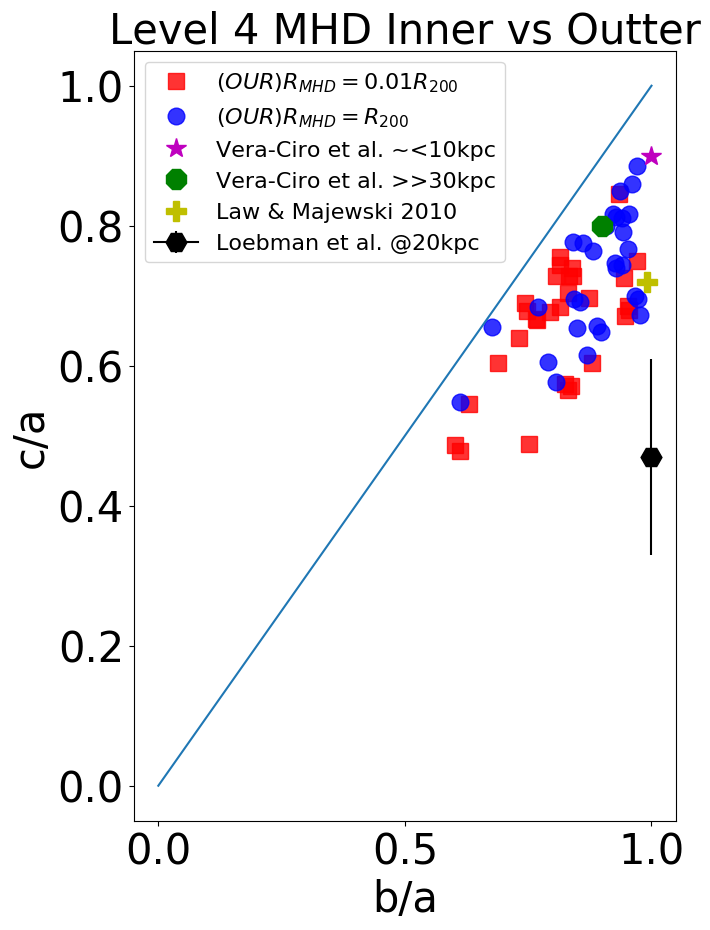
\includegraphics[width=0.5\columnwidth]{./pics/Triaxial_Plane/Triaxiality_MHD_lvl4.png}}
  \hfill
  \caption{General tendency on the triaxial plane $c/a$ Vs $b/a$. Some observational constraints are plotted alongside our results (Optimize space. caption replaces title.  Present constraints representation of density)}
  \label{fig:Triaxiality_DM_MHD}
\end{figure}

\subsection{The rounding effect of baryons}
Here we discuss the rounding effect of baryons. We quantify this rounding effect and look for correlations with important baryonic properties of the galaxy.

\begin{figure}
  \centering
  \subfloat[Level4 MHD Vs DM at inner regions]{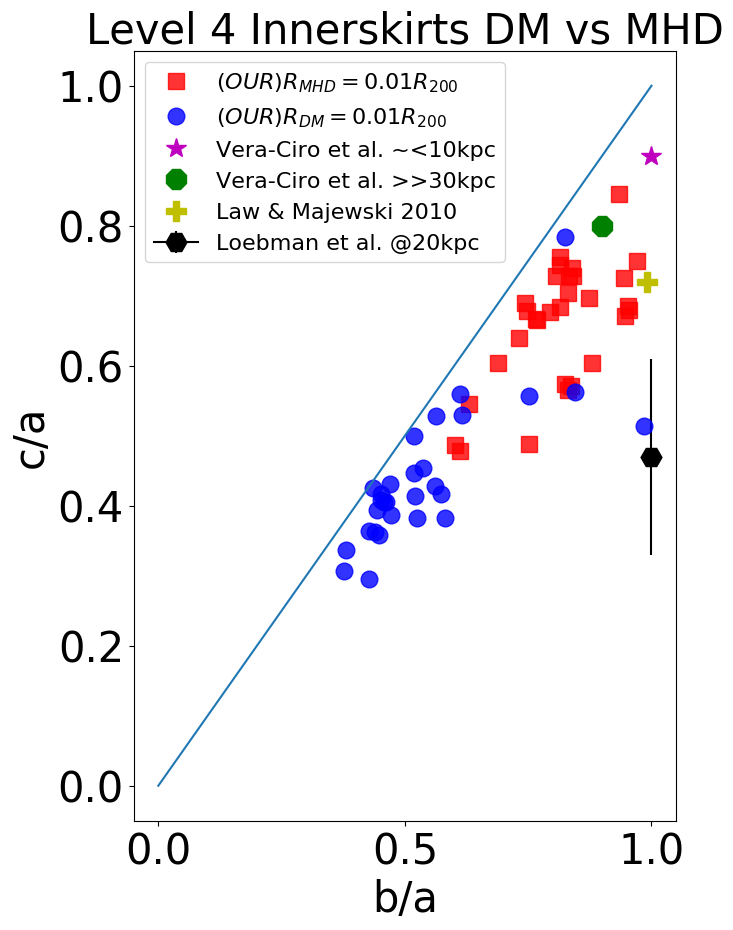
\includegraphics[width=0.5\columnwidth]{./pics/Triaxial_Plane/Triaxiality_Inner_lvl4.png}}
  \hfill
  \subfloat[Level4 MHD Vs DM at outer regions]{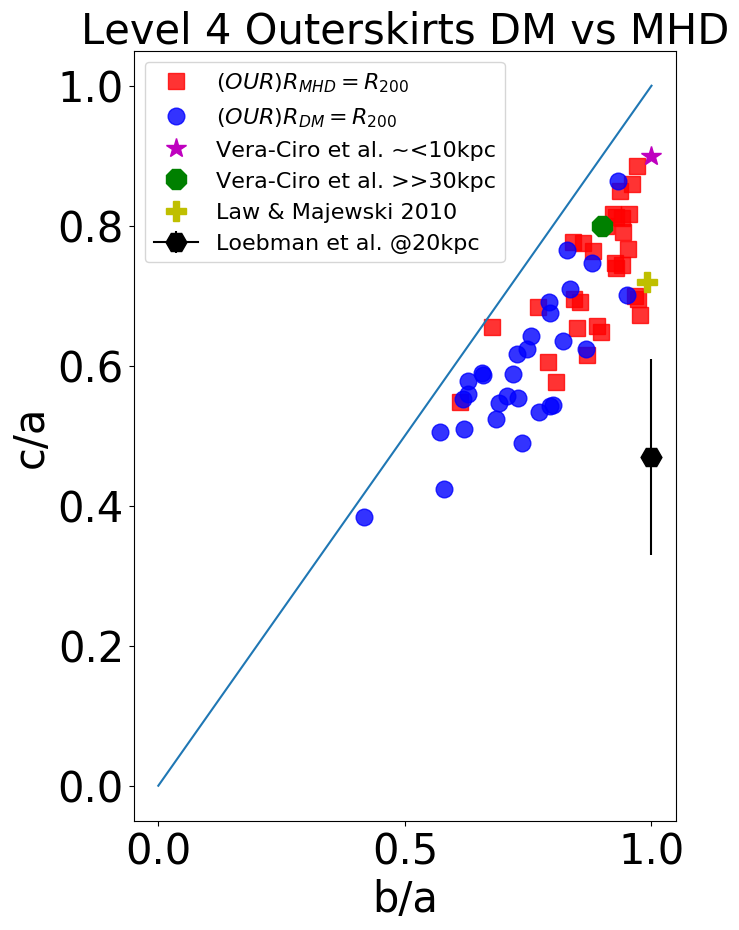
\includegraphics[width=0.5\columnwidth]{./pics/Triaxial_Plane/Triaxiality_Outter_lvl4.png}}
  \hfill
  \caption{Axial ratios as shown on $c/a$ Vs $b/a$. Each dot represents a halo shape at some radius. Some observational constraints are plotted alongside our results. Here, dots are clustered, proving the general tendence of halos to get rounder on the outer parts.(Optimize space. caption replaces title.  Present constraints representation of density)}
  \label{fig:Triaxiality_Inner_Outer}
\end{figure}

\begin{figure}
	% To include a figure from a file named example.*
	% Allowable file formats are eps or ps if compiling using latex
	% or pdf, png, jpg if compiling using pdflatex
	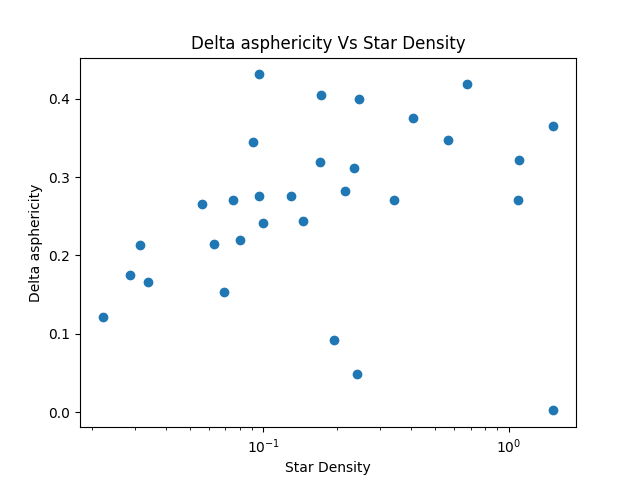
\includegraphics[width=\columnwidth]{./pics/Delta asphericity Vs Star Density.png}
    \caption{Difference in asphericities between MHD and DM shapes Vs Star Density of the simulation.}
    \label{fig:Star_Density_effect}
\end{figure}

\subsection{The historical shape}
Here we study the memory shape and how it can be deduced from the historic radial shapes. Also why it is lost for MHD even when radial profiles have the same historic tendencies.

\begin{figure}
  \centering
  \subfloat[halo 16 DM]{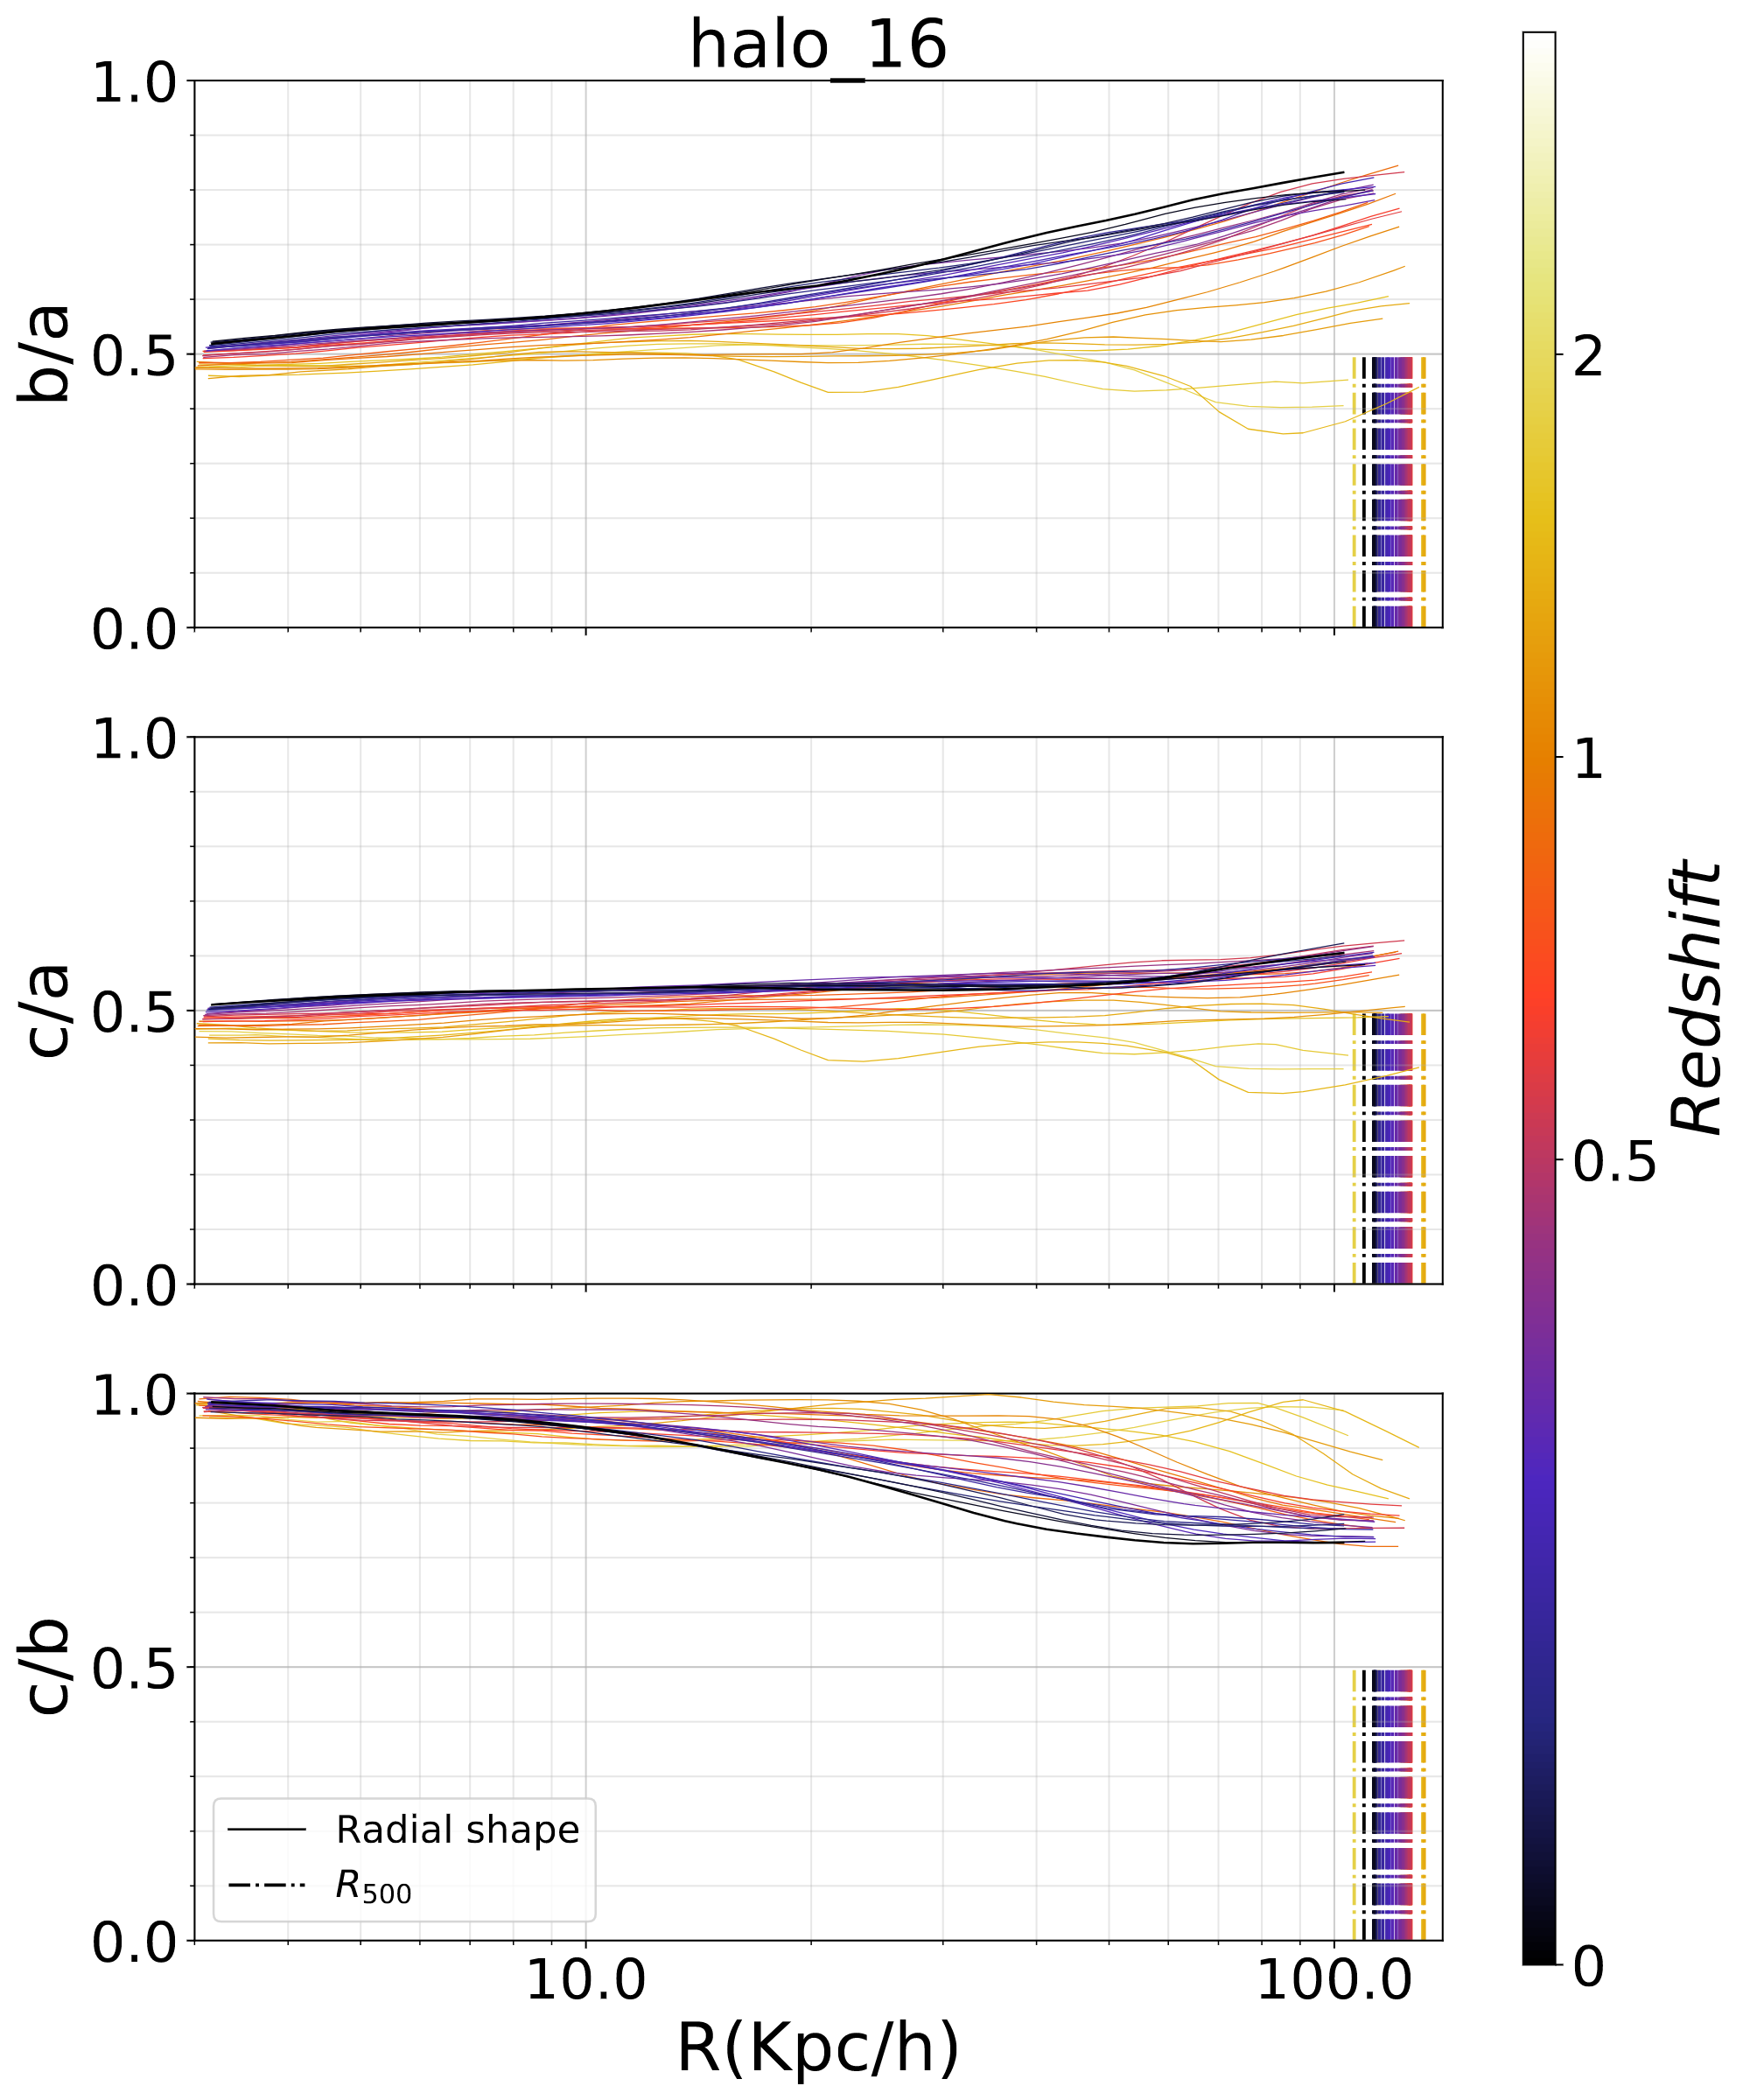
\includegraphics[width=0.5\columnwidth]{./pics/Redshift/halo_16_level3_DM_Z.png}}
  \hfill
  \subfloat[halo 16 MHD]{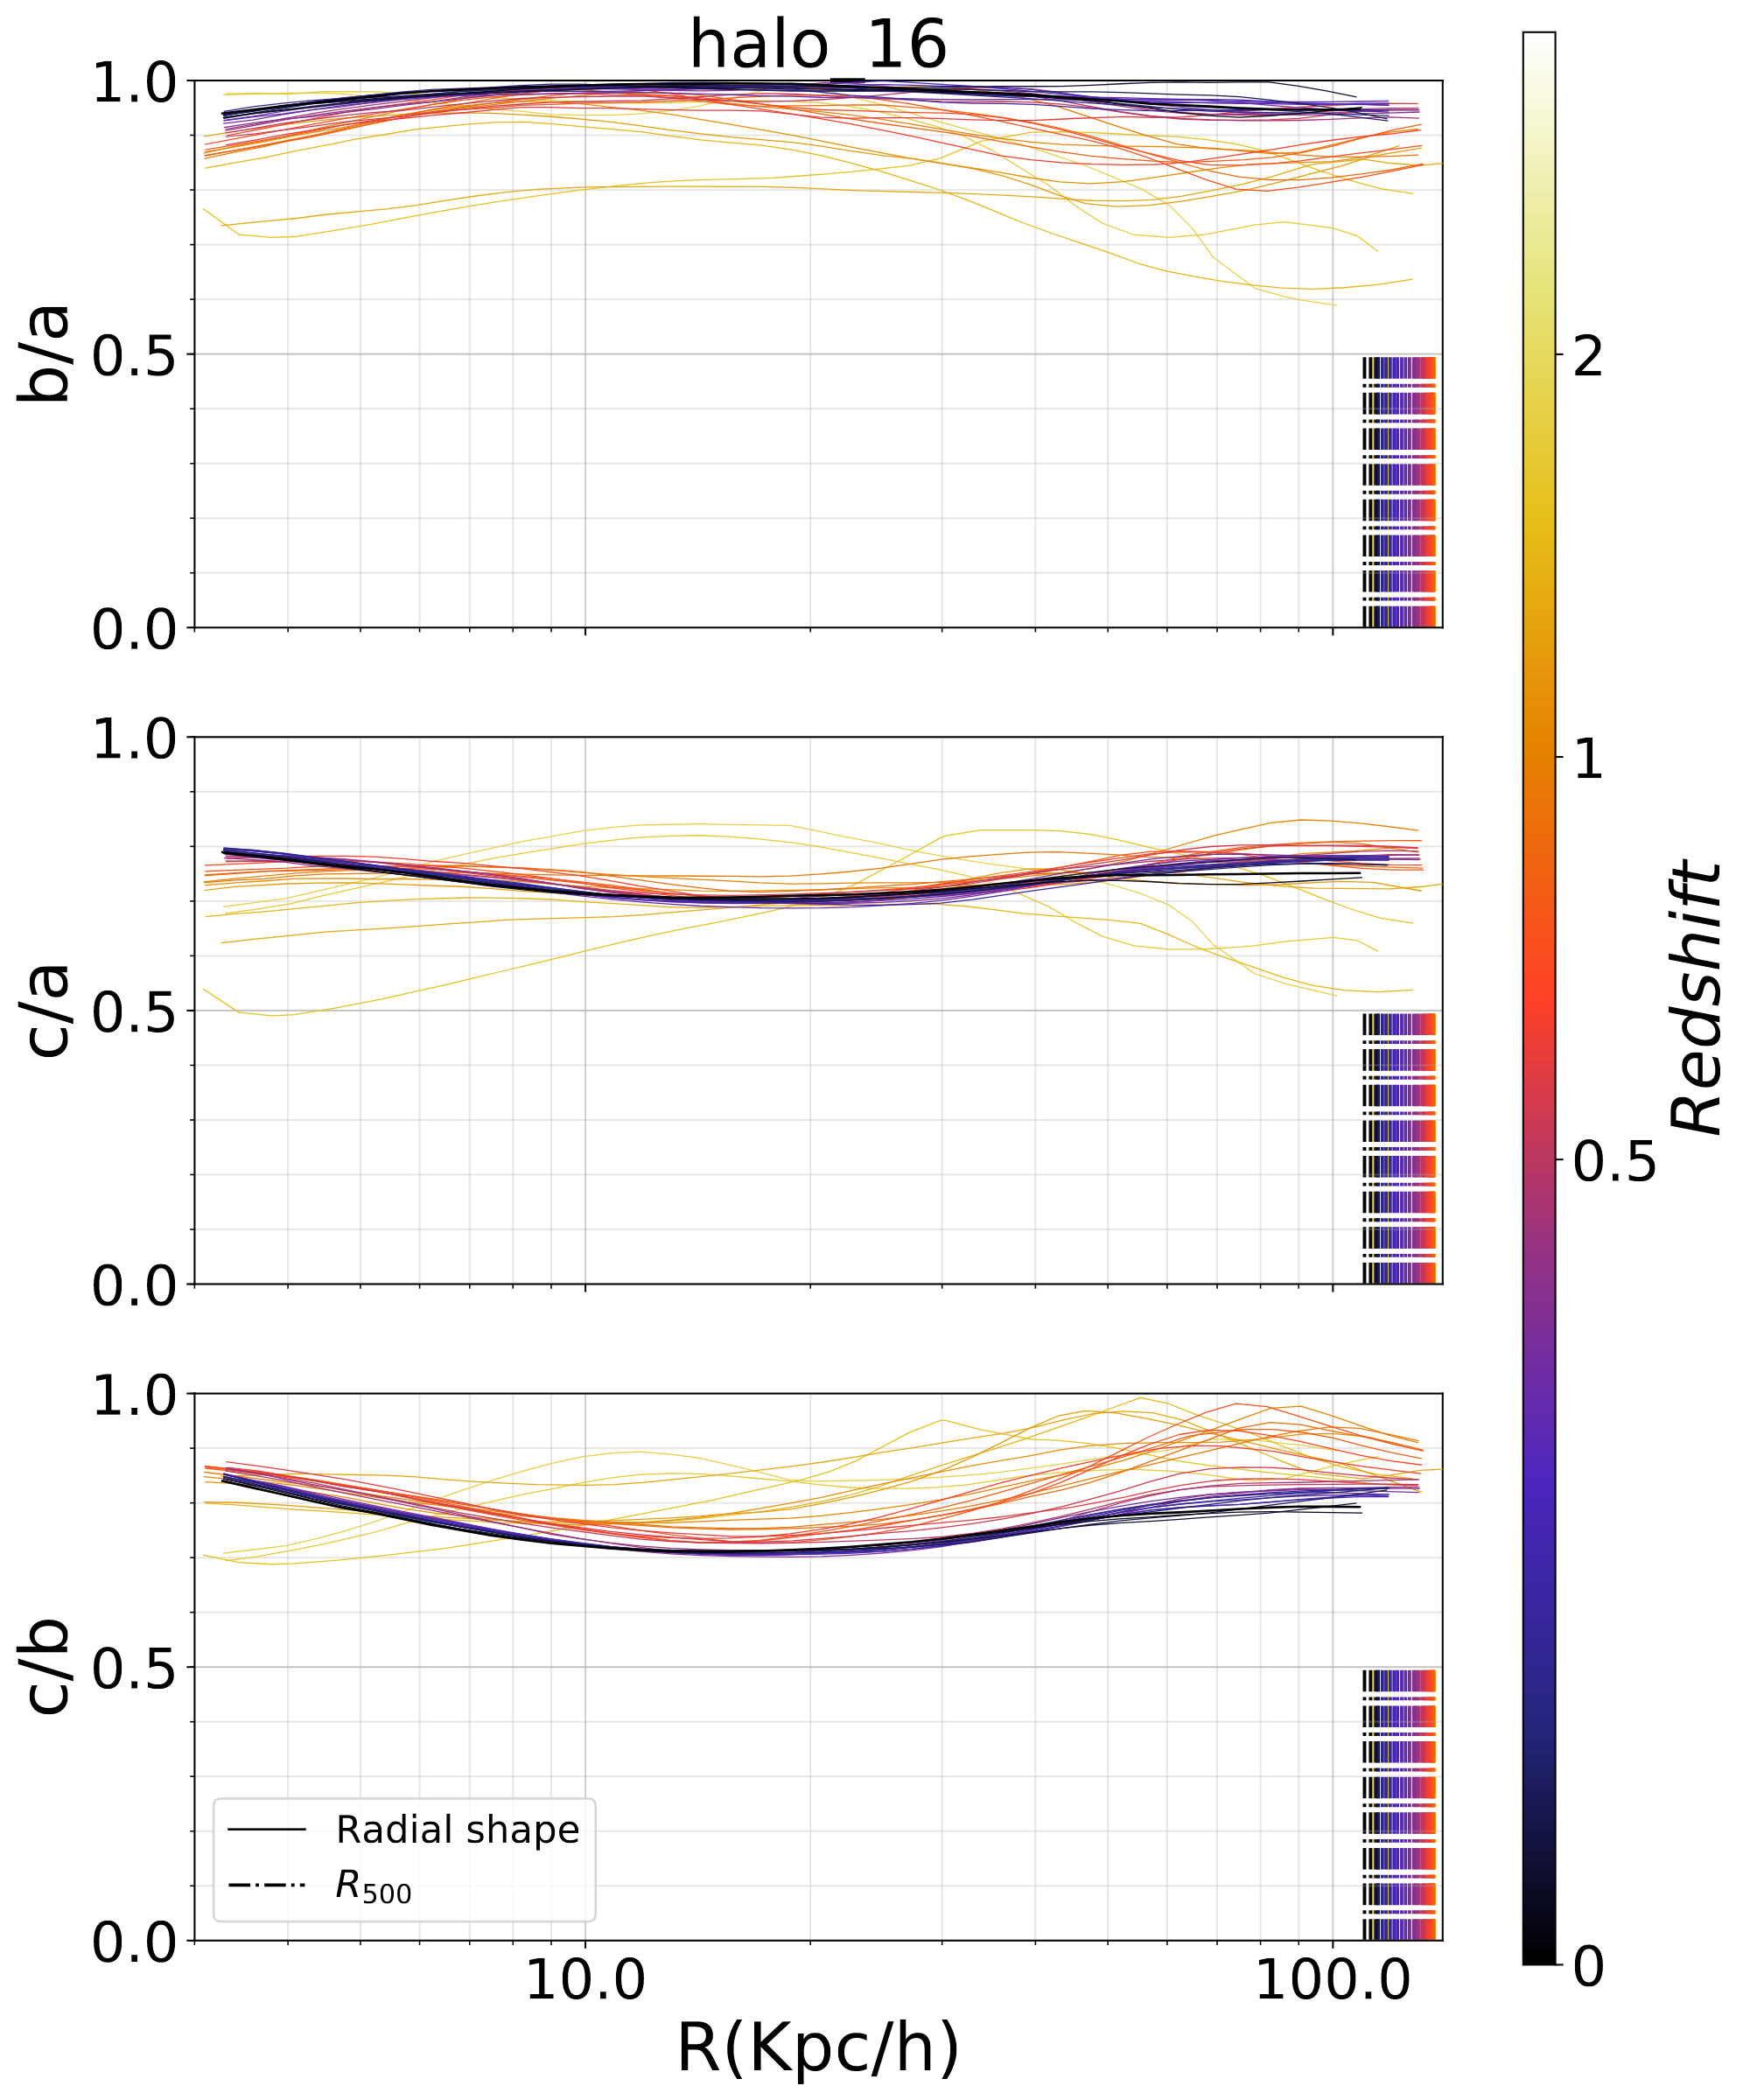
\includegraphics[width=0.5\columnwidth]{./pics/Redshift/halo_16_level3_MHD_Z.png}}
  \caption{Radial profile (comoving) of axial ratios for halo 16 in terms of redshift (color). This halo maintains its shape until $z\approx 1$ obviating the systematic rounding effect in time from asymmetric potentials. }
  \label{fig:RedshiftGood}
\end{figure}

\subsection{The orientation of the principa axes}
This is an important result of our study. We study the radial evolution of the principal axes, compared also to the angular momentum vector from the disk. We found that while the angular momentum tend to be aligned with the minor axis of the ellipsoid, this may not be the case all times. When there is an alignment it is usually within 20 degrees. When there is not an alignment, then there is no simple way to determine toward which axis it is oriented. Furthermore, the principal axes alignment usually change with radius (rotation, swap). This really questions the strong constrains on the MW DM halo models. 


\begin{figure}
  \centering
  \subfloat[Aligned Axes]{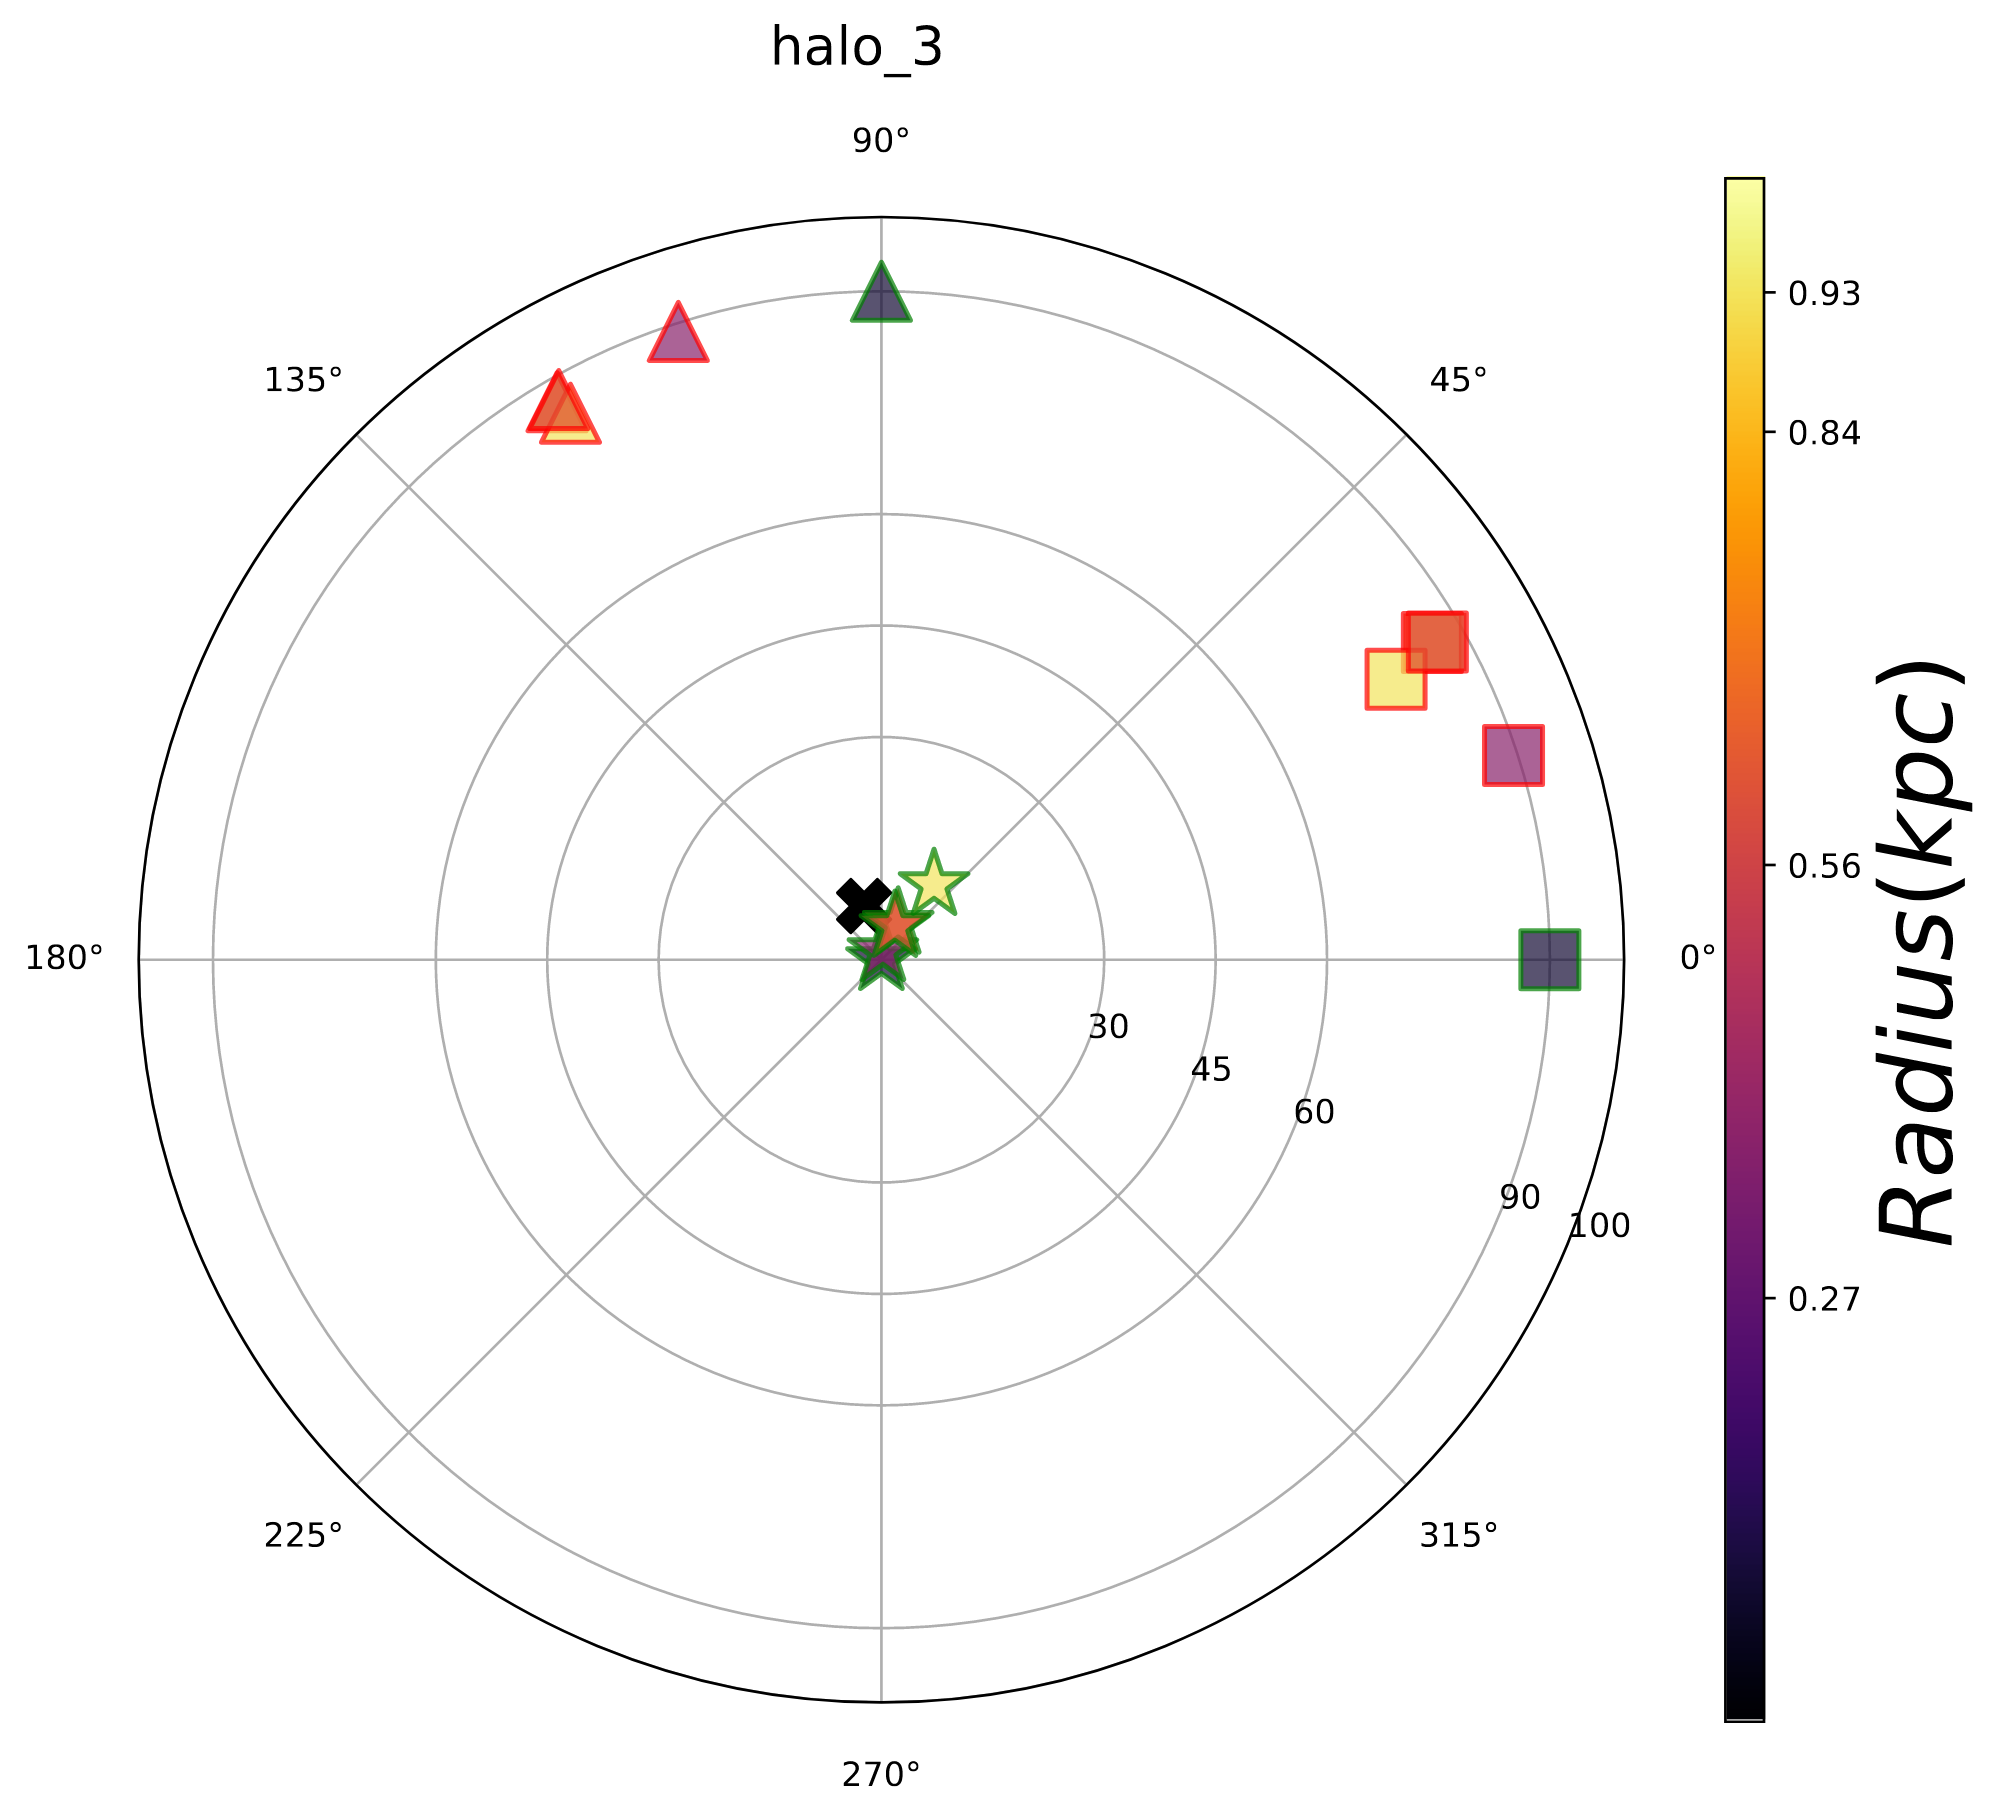
\includegraphics[width=1\columnwidth]{./pics/well_axes.png}}
  \hfill
  \subfloat[Rotating Axes]{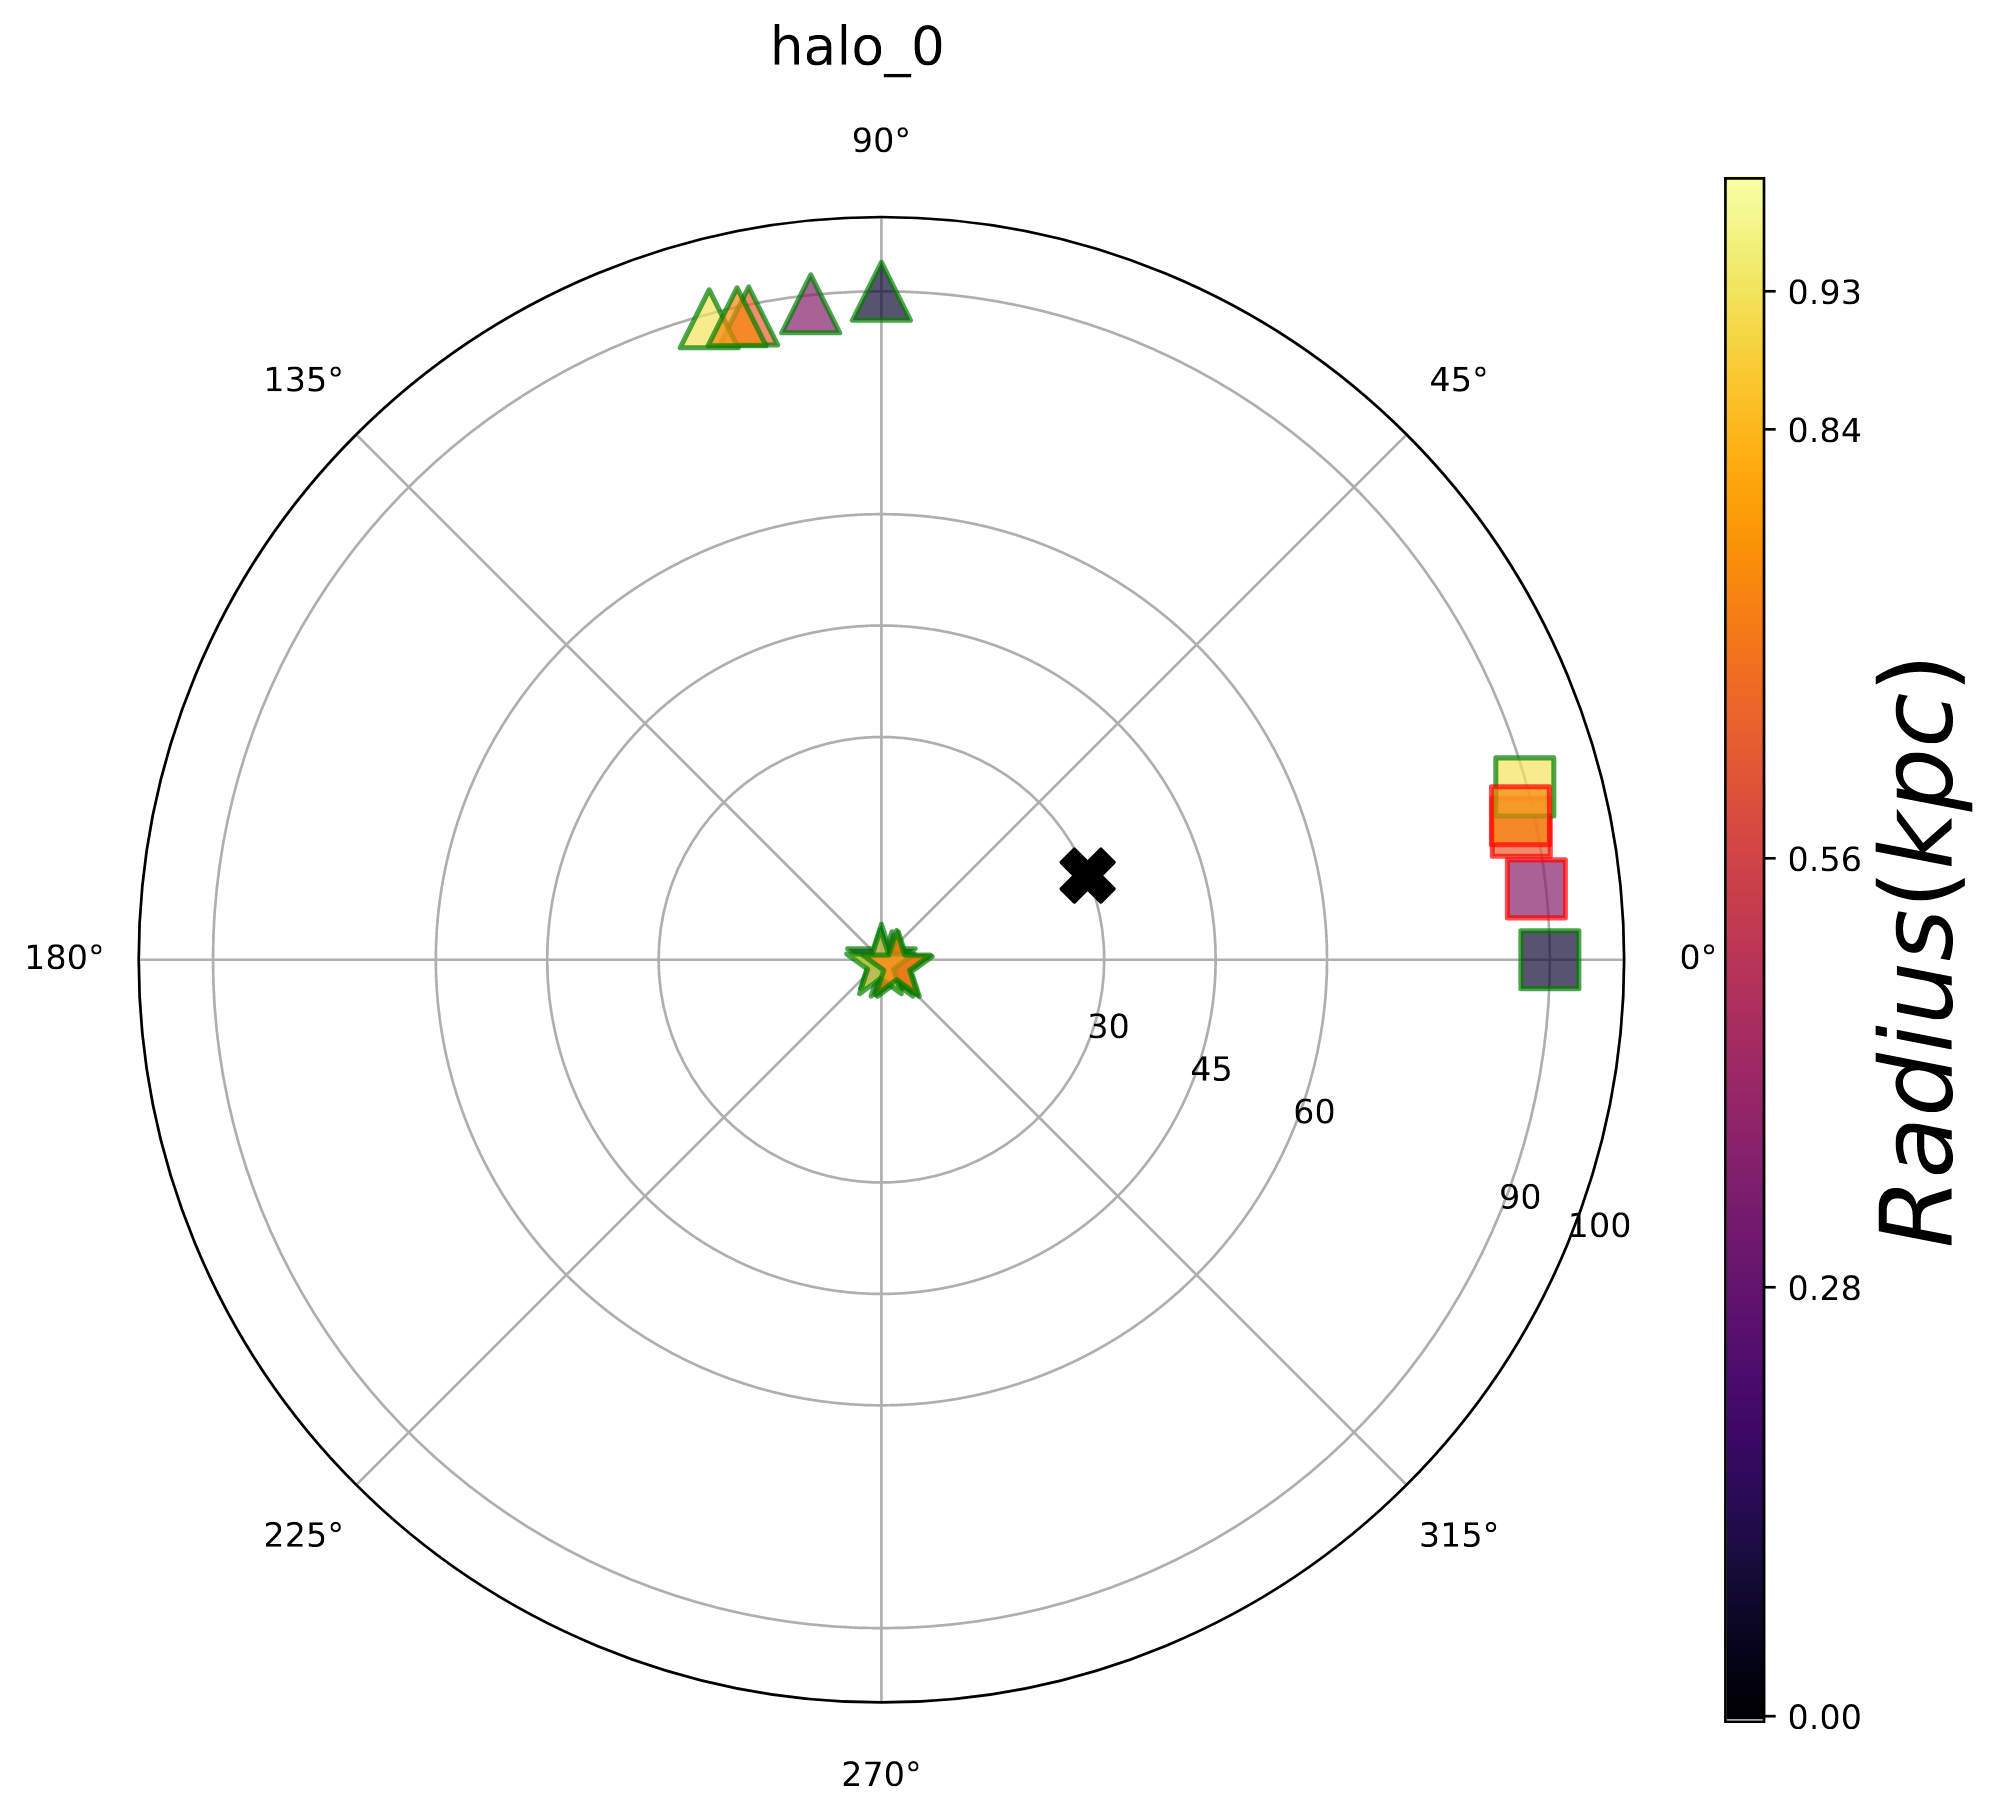
\includegraphics[width=1\columnwidth]{./pics/rotating_axes.png}}
  \hfill
  \subfloat[Chaotic Axes]{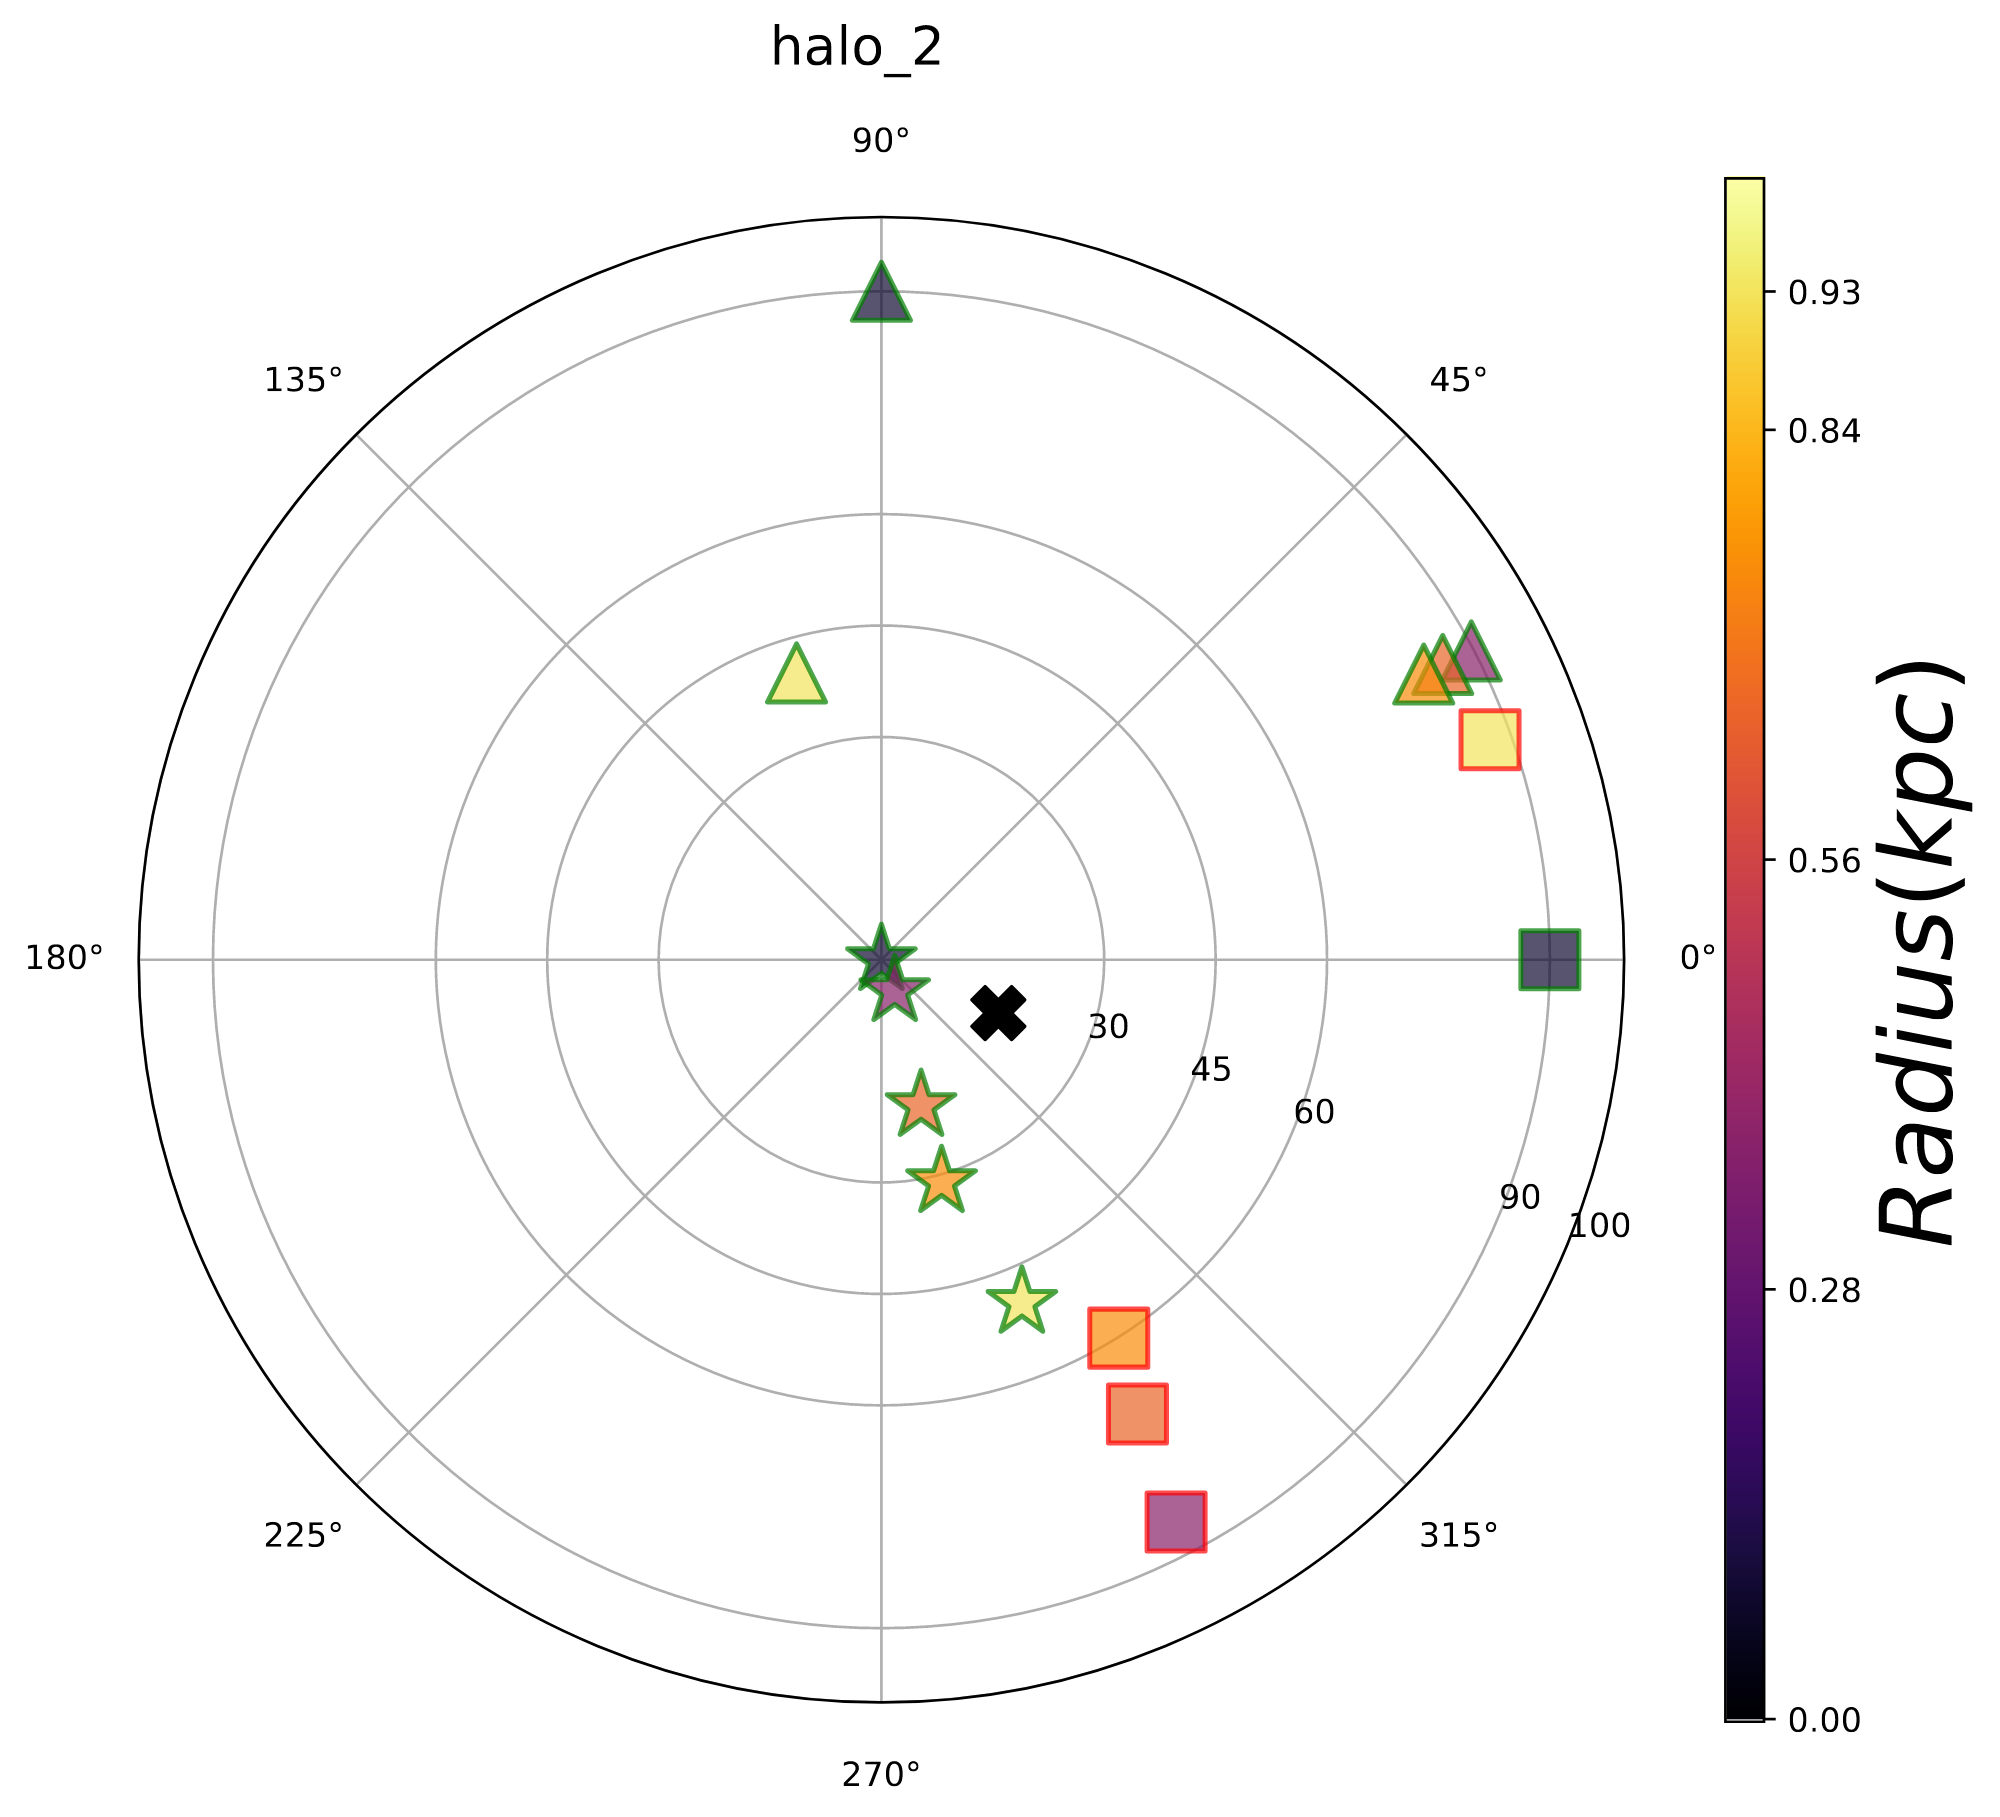
\includegraphics[width=1\columnwidth]{./pics/chaotic_axes.png}}
  \hfill
  \caption{Description of axes alignments }
  \label{fig:slices}
\end{figure}



\section{Conclusions}

The last numbered section should briefly summarise what has been done, and describe
the final conclusions which the authors draw from their work.

\section{Discussion}

\section*{Acknowledgements}



The Acknowledgements section is not numbered. Here you can thank helpful
colleagues, acknowledge funding agencies, telescopes and facilities used etc.
Try to keep it short.

%%%%%%%%%%%%%%%%%%%%%%%%%%%%%%%%%%%%%%%%%%%%%%%%%%

%%%%%%%%%%%%%%%%%%%% REFERENCES %%%%%%%%%%%%%%%%%%

% The best way to enter references is to use BibTeX:

%\bibliographystyle{mnras}
%\bibliography{example} % if your bibtex file is called example.bib


% Alternatively you could enter them by hand, like this:
% This method is tedious and prone to error if you have lots of references
\begin{thebibliography}{99}
\bibitem[\protect\citeauthoryear{Author}{2012}]{Author2012}
Author A.~N., 2013, Journal of Improbable Astronomy, 1, 1
\bibitem[\protect\citeauthoryear{Others}{2013}]{Others2013}
Others S., 2012, Journal of Interesting Stuff, 17, 198
\end{thebibliography}

%%%%%%%%%%%%%%%%%%%%%%%%%%%%%%%%%%%%%%%%%%%%%%%%%%

%%%%%%%%%%%%%%%%% APPENDICES %%%%%%%%%%%%%%%%%%%%%

\appendix

\section{Some extra material}

If you want to present additional material which would interrupt the flow of the main paper,
it can be placed in an Appendix which appears after the list of references.

%%%%%%%%%%%%%%%%%%%%%%%%%%%%%%%%%%%%%%%%%%%%%%%%%%


% Don't change these lines
\bsp	% typesetting comment
\label{lastpage}
\end{document}

% End of mnras_template.tex